\documentclass{article}

\usepackage{geometry}
\usepackage[T1]{fontenc}
\usepackage[utf8]{inputenc}
\usepackage{amssymb}
\usepackage{amsmath}
\usepackage{amsfonts}
\usepackage{ngerman}
\usepackage{pgf}
\usepackage{listings}
\usepackage{graphicx}
\graphicspath{ {Bilder/} }

\usepackage{tikz}
\usetikzlibrary{arrows, automata, matrix}
\usetikzlibrary{positioning}

\usepackage{color}

\usepackage{hyperref}

\newcommand{\kreis}[1]{\unitlength1ex\begin{picture}(2.5,2.5)%
	\put(0.75,0.75){\circle{2.5}}\put(0.75,0.75){\makebox(0,0){#1}}\end{picture}}

\lstdefinestyle{customc}{  % Config der lstlisting Umgebung
	belowcaptionskip=1\baselineskip,
	breaklines=true,
	frame=single,
	xleftmargin=\parindent,
	language=C++,
	showstringspaces=false,
	basicstyle=\footnotesize\ttfamily,
	keywordstyle=\bfseries\color{green!40!black},
	commentstyle=\itshape\color{purple!40!black},
	identifierstyle=\color{blue},
	stringstyle=\color{orange},
}
\lstset{literate=  % Sonderzeichen in lstlisting Umgebung
	{á}{{\'a}}1 {é}{{\'e}}1 {í}{{\'i}}1 {ó}{{\'o}}1 {ú}{{\'u}}1
	{Á}{{\'A}}1 {É}{{\'E}}1 {Í}{{\'I}}1 {Ó}{{\'O}}1 {Ú}{{\'U}}1
	{à}{{\`a}}1 {è}{{\`e}}1 {ì}{{\`i}}1 {ò}{{\`o}}1 {ù}{{\`u}}1
	{À}{{\`A}}1 {È}{{\'E}}1 {Ì}{{\`I}}1 {Ò}{{\`O}}1 {Ù}{{\`U}}1
	{ä}{{\"a}}1 {ë}{{\"e}}1 {ï}{{\"i}}1 {ö}{{\"o}}1 {ü}{{\"u}}1
	{Ä}{{\"A}}1 {Ë}{{\"E}}1 {Ï}{{\"I}}1 {Ö}{{\"O}}1 {Ü}{{\"U}}1
	{â}{{\^a}}1 {ê}{{\^e}}1 {î}{{\^i}}1 {ô}{{\^o}}1 {û}{{\^u}}1
	{Â}{{\^A}}1 {Ê}{{\^E}}1 {Î}{{\^I}}1 {Ô}{{\^O}}1 {Û}{{\^U}}1
	{œ}{{\oe}}1 {Œ}{{\OE}}1 {æ}{{\ae}}1 {Æ}{{\AE}}1 {ß}{{\ss}}1
	{ű}{{\H{u}}}1 {Ű}{{\H{U}}}1 {ő}{{\H{o}}}1 {Ő}{{\H{O}}}1
	{ç}{{\c c}}1 {Ç}{{\c C}}1 {ø}{{\o}}1 {å}{{\r a}}1 {Å}{{\r A}}1
	{€}{{\euro}}1 {£}{{\pounds}}1 {«}{{\guillemotleft}}1
	{»}{{\guillemotright}}1 {ñ}{{\~n}}1 {Ñ}{{\~N}}1 {¿}{{?`}}1
}
\lstset{style=customc, tabsize=2}
\tikzset{
	state/.style={
			rectangle, rounded corners,
			draw=black,  thick, minimum height=2em, inner sep=2pt, text centered},
		}

\begin{document}
	
	\tableofcontents
	\newpage
	
	\section{Rechenoperationen}
	\label{beispiel}
	\begin{enumerate}
		\item Baum besteht aus Knoten (Kreise) und Kanten (Pfeile)
		\item Kanten verbinden Knoten mit ihren Kind-Knoten
		\item jeder Knoten (außer der Wurzel) hat \underline{genau ein} Elternteil
		\item Knoten ohne Kinder heißen "'Blätter"' (leaf-nodes)
		\item Teilbaum
		\begin{enumerate}
			\item wähle beliebigen Knoten
			\item entferne temporär dessen Eltern-Kante
			\begin{enumerate}
				\item der Knoten wird temorär zu einer Wurzel
				\item dieser Knoten mit allen seinen Nachkommen bildet wieder seinen Baum - "' Teilbaum des Originalbaums"'
			\end{enumerate}
			\item Tiefe: Abstand des Knotens zur Wurzel
			\item 
		\end{enumerate}
	\end{enumerate}
	
	Infix-Notation: \\
	 $1+2+3*4/(1+5)-2$ \\ \\
	 Präfix-Notation: \\
	 $sub(add(add(1,2), div(mul(3,4), add(1,5))),2)$ \\ \\
	 
	 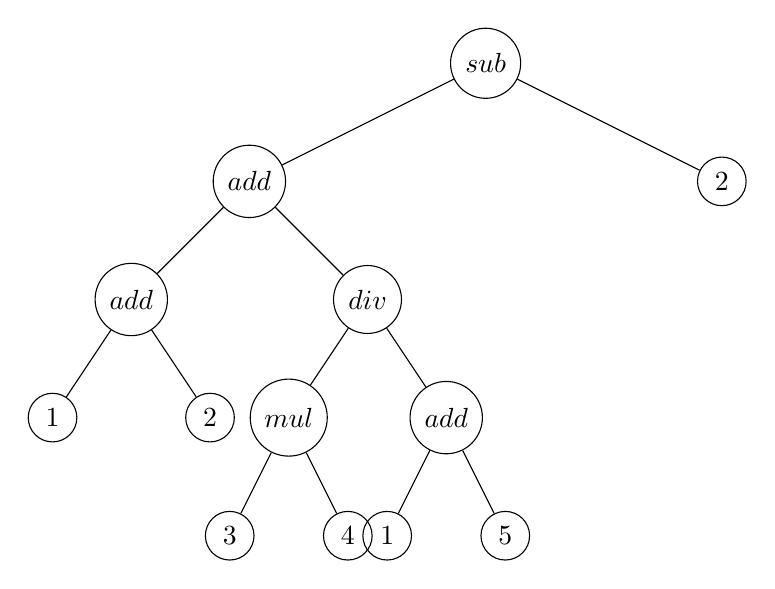
\begin{tikzpicture}[level/.style={sibling distance=60mm/#1}]
	 	
	 	\node [circle, draw] (z)  {$sub$}
	 	child {node [circle, draw] {$add$}
	 		child {node [circle, draw] {$add$}
	 			child{node [circle, draw] {$1$}}
	 			child{node [circle, draw] {$2$}}
	 		}
	 		child {node [circle, draw] {$div$}
	 			child{node [circle, draw] {$mul$}
	 				child {node [circle, draw] {$3$}}
	 				child {node [circle, draw] {$4$}}
	 			}
	 			child{node [circle, draw] {$add$}
	 				child {node [circle, draw] {$1$}}
	 				child {node [circle, draw] {$5$}}
	 			}
	 		}}
	 		child {node [circle, draw] {$2$}
	 		};
	 	\end{tikzpicture}
	 		
	\paragraph{Präfix Notation aus dem Baum rekonstruieren}
	 		
	 \begin{enumerate}
	 	\item Wenn die Wurzel ein Blatt ist, dann "'Drucke die Zahl"'
	 	\item sonst (Operator):
	 	\begin{enumerate}
	 		\item Drucke Funktionsnamen
	 		\item Drucke "'("'
	 		\item wiederhole ab $1)$ für das linke Kind
	 		\item Drucke "',"'
	 		\item wiederhole den Algorithmus ab $1)$ für das rechte Kind
	 		\item Drucke "')"'
	 	\end{enumerate}
	 \end{enumerate}
	
		Beachte Reihenfolge: Wurzel - Links - Rechts (Pre-Order Traversal)
		Ergebnis: \\
		$sub(add(add(1,2), div(mul(3,4), add(1,5))),2)$
		
		\paragraph{Definition: Rekursion}
		Rekursion meint Algorithmus für Teilproblem von vorn
		
		\paragraph{Infix Notation}
		
		\begin{enumerate}
			\item wie bei Präfix
			\item sonst
			\begin{enumerate}
				\item entfällt
				\item wie bei Präfix
				\item wie bei Präfix
				\item Drucke Operatorsymbol
				\item wie bei Präfix 
				\item wie bei Präfix
				\item wie bei Präfix
			\end{enumerate}
		\end{enumerate}
		Beachte Reihenfolge: Links - Wurzel - Rechts (In-Order Traversal) \newline
		
		Ergebnis: \\
		$(((1 + 2) + ((3 * 4)/(1 + 5))) + 2)$
		
		\paragraph{Berechne den Wert mit Substitutionsmethode}
		\begin{enumerate}
			\item Wenn Wurzel ein Blatt hat, gib die Zahl zurück
			\item sonst
			\begin{enumerate}
				\item entfällt
				\item entfällt
				\item wiederhole ab $1)$ für linken Teilbaum und speichere Ergebnis als "'left-result"'
				\item entfällt
				\item wiederhole ab $1)$ für rechten Teilbaum, speichere Ergebnis als "'right-result"'
				\item berechne $fkt_name(left-result, right-result)$ und gib Ergebnis zurück
			\end{enumerate}
		\end{enumerate}
		Beachte Reihenfolge: Links - Rechts - Wurzel (Post-Order Traversal)
		
		\begin{align*}
		&  	sub(add(add(1,2), div(mul(3,4), add(1,5))),2) \\
		= & \, sub(add(add(1,2), div(12, 6)),2) \\
		= & \, sub(add(3,2)2) \\
		= & \, sub(5,2) \\
		= & \, 3
		\end{align*}
		
		\section{Maschinensprache}
		\begin{itemize}
			\item optimiert für die Hardware (viele verschiedene)
			\item Gegensatz: höhere Programmiersprache ($C++$) ist optimiert für Programmierer
			\item Compiler oder Interpreter übersetzen Hoch- in Maschinensprache 
		\end{itemize}
		
		\paragraph{Vorgang des Übersetzens}
		\begin{enumerate}
			\item Eingaben (und Zwischenergebnisse) werden in Speicherzellen abgelegt $ \Rightarrow$ jeder Knoten im Baum bekommt eine Speicherzelle (Maschinensprache: durchnumeriert ; Hochsprache: sprechende Namen)
			\item Speicherzellen für die Eingaben $\underline{initialisieren}$ ; Notation: SpZ $\leftarrow$ Wert
			\item Rechenoperationen in der Reihenfolge des Substitutionsmodells ausführen und in der jeweiligen Speicherzelle speichern ; Notation: SpZ\_Ergebnis $\leftarrow$ fkt\_name SpZ\_Arg1 SpZ\_Arg2
			\item alles in Zahlencode umwandeln
			\begin{itemize}
				\item Funktionsname $\Rightarrow$ Opcodes
				\item Speicherzellen: nur die Nummer
				\item Werte sind schon Zahlen
				\item Notation: Opcode \quad Ziel SpZ \quad SpZ\_Arg1 \quad SpZ\_Arg2 oder Opcode \quad Ziel SpZ \quad Initialwert
			\end{itemize}
		\end{enumerate}
	
	\section{funktionale Programmierung}
	(alles durch Funktionsaufrufe ausführen)
	
	\begin{enumerate}
		\item bei Maschinensprache wurden Zwischenergebnisse in Speicherzellen abgelegt
		\item das ist auch in der funktionalen Programm. eine gute Idee
		\begin{enumerate}
			\item Speicherzellen werden durch Namen (vom Programmierer vergeben) unterschieden
			\item Beispiel: Lösen einer quadratischen Gleichung: $ax^2+bx+c =0$, finde $x_{1/2}$
					$\Rightarrow x^2-px+q =0 \quad mit \quad p = -\frac{b}{2a}, q = \frac{c}{a}$
					$\Rightarrow x_1 = -\frac{b}{2a} + \sqrt{(-\frac{b}{2a}^2 - \frac{c}{a})} \\ \Leftarrow allgemein: x_{1/2} = p \pm \sqrt{p^2-q}$
			\item Präfix: \\ $x_1 \leftarrow add(div(div(b,a),-2), sqrt(sub(mul(div(div(b,a),-2), div(div(b,a), -2)), div(c,a))))$ \\
					mit Zwischenergebnissen und Infix-Notation: $p \leftarrow b/c/-2 \quad $oder$ \quad p \leftarrow -0,5*b/a \quad q \leftarrow c/a$ \\ $discriminant \leftarrow sqrt(p*P-q)$ \\
					$x_{1/2} \leftarrow p \pm discriminant$
		\end{enumerate}
		\item zwei Vorteile:
		\begin{enumerate}
			\item lesbar
			\item redundante Berechnung verschieden \\ Beachte: In der funktionalen Programmierung können die Speicherzellen nach der Initialisierung \underline{nicht} mehr verändert werden
			\item Speicherzellen mit Namen sind nützlich, um Argumente an Funktionen zu übergeben $\Rightarrow$ Definition eigener Funktionen \\
			Bsp: 
			\framebox{function sq(x) \\
												\{
												return x*x
												\} }
		\end{enumerate}
	\end{enumerate}
	
	\section{funktionale Programmierung in C++}
	
	\begin{enumerate}
		\item in C++ hat jede Speicherzelle einen \underline{Typ} (legt Größe und Bedeutung der Speicherzelle fest) \\
		wichtigste Typen: \grqq int\grqq  für ganze Zahlen, \grqq double\grqq  für reelle Zahlen, \grqq std::string\grqq  für Text \\ zugehörige Literale (Konstanten): 12, -3 (int) \quad -1.02 , 1.2e-4 (double) \quad \grqq text text \grqq (string)
		\item Die Initialisierung wird geschrieben als
		\begin{lstlisting}[tabsize =2]
			type_name spz_name = initialwert
		\end{lstlisting}
		Bsp:
		\begin{lstlisting}[tabsize = 2]
			double a = 10
			std::cout << "x_1" << x_1 << "\n" ;
		\end{lstlisting} 
		\item eigene Funktion in $C++$: 

			\begin{lstlisting}[tabsize = 2]
			type_ergebnis funktionsname (typ_arg1 name_arg1, typ_arg2 name_arg2)
			{
				<code>
				return ergebnis;
			}
			\end{lstlisting}
			
		\item zwei Funktionen mit gleichem Namen, aber unterschiedlichen Typen dürfen in C++ gleichzeitig definiert sein (\grqq overloading\grqq) \\ $\Rightarrow$ C++ wählt \underline{automatisch} die richtige Variante anhand des Argumenttypes (\grqq overload resolution\grqq)
		
		\item jedes $C++$ -Programm muss \underline{genau eine} Funktion names \grqq main\grqq haben: Dort beginnt die Programm-Ausführung \\
		Bsp: \\
		\fbox{\centering int main() \{ <code> \quad return 0 (erfolgreich abgearbeitet)\}}
		
		\item Regel von $C++$ für erlaubte Namen (Speicherzelle \& Funktion):
		\begin{enumerate}
			\item erste Zeichen: Klein- oder Großbuchstaben des englischen Alphabets oder \_
			\item optional: weitere Zeichen: wie erstes Zeichen oder Ziffern 0 \dots 9
		\end{enumerate}
		
		\item vordefinierte Funktionen in $C++$
		\begin{enumerate}
			\item eingebaute Funktionen (immer vorhanden) z.B. Infix Operatoren
			\item Funktionen der Standardbibliothek (Programmierer muss sie explizit auffordern)
			\begin{enumerate}
				\item z.B. algebraische Funtionen beginnend mit std::\dots
				\item sind in Module geordnet, z.B. cmath $\widehat{=}$ \, algebraische Funktionen, iostream $\widehat{=}$ \, Ausgabe, z.B. std::cout
				\item Um ein Modul zu benutzen, muss man zuerst (am Anfang des Programms) sein Inhaltsverzeichnis importieren \\
				\frame{\centering \#include <module\_name>} sprich \grqq Header inkludieren\grqq \\
				 \\
			\end{enumerate}
		\end{enumerate}
	\end{enumerate}
	
	\begin{lstlisting} [tabsize = 2]
	# include <iostream> 
	# include <string> 
	
	int main() {
	
	std::cout <<  "Hello" << "\n";
	std::string >> ausgabe = "mein erstes Programm"
	std::cout << ausgabe;
	
	return 0
	}
	\end{lstlisting}
	
	\subsection{Overloading der arithmetischen Operationen}
	
	\begin{lstlisting} [tabsize = 2]
		int a = 3;
		int b = 4;
		int c = a * b;
		double x = 3.0;
		double y = 4.0;
		double z = x * y;
	\end{lstlisting}
	$3.0 * 4 \quad \Rightarrow \quad$ automatische Umwandlung in höheren Typ, hier: \grqq double\grqq $\Rightarrow$ wird als $3.0 * 4.0$ ausgeführt \\
	
	\subsection{Interger-Division in $C++$}
	
	Konsequenzen:
	\begin{enumerate}
		\item Division unterscheidet sich nach dem Datentypen: $(-12)/5 \Rightarrow -2 \neq -2.4 \Leftarrow (-12.0/5.0)$
		\item negative Ereignisse werden aufgerund, positive abgerundet (truncating division) \\
				d.h. Nachkommstellen abschneiden, d.h. Richtung Null runden
		\item Gegensatz (z.B. zu Python): floor division $\widehat{=}$ wird immer abgerundet
		\item Divisionsrest: 
			\end{enumerate}
		\begin{lstlisting} [tabsize = 2]
			int a = ...;
			int b = ...;
			int q = a/b;
			(a/b)*b = q * b
		\end{lstlisting}
		ist im allgemeinen \underline{ungleich} $a$ $\Rightarrow$ 
		\begin{lstlisting} [tabsize = 2]
			int rest = a = q*b;
		\end{lstlisting}
		\begin{enumerate}
		\item wenn Division aufgeht $\Rightarrow$ rest = 0 , sonst $\neq 0$
		\item Invariante: 
		\begin{lstlisting} [tabsize = 2]
			(a/b) * b + rest = a
			
			int rest1 = a % b;  // aequivalent: a-(b/a)*b
		\end{lstlisting}
	\end{enumerate}
	
	\subsection{Anwendung}
	
	Wochentag für beliebiges Datum bestimmen:
	gegeben: $d,m,y$ , gesucht: $w \in \{0,\dots , b\}$ \\
		int weekday(int d, int w, int y) {}  ; weekday(10,11,2016) $\Rightarrow$ 3 (Donnerstag)
		
		Teilprobleme
		\begin{enumerate}
				\item finde den Wochentag vom 1. Januar y
				\item finde den Abstand vom (d,m,y) zum (1,1,y)
				\item setze beides zusammen \\

		\end{enumerate}
		
	Schaltjahresregel: y ist Schaltjahr, wenn:
	\begin{enumerate}
		\item y durch 4 teilbar, aber nicht durch 100 $\Rightarrow$ 2004, 2006, nicht 2100
		\item y durch 400 teilbar $\Rightarrow$ 2000 \\ \\
		 $\Rightarrow$ 400-Jahres-Zyklus der Regeln: nach 400 Jahren beginnt die Schaltjahresregel von vorn
 	\end{enumerate}
 	
 	\begin{itemize}
 		\item Beobachtung: der 1.1.2001 ist der erste Tag eines neuen Zyklus und war Montag
 		\item die Anzahl der Tage vom 1.1.y zum 1.1.2001 ist: \\
 		$z = y - 2001 \quad \triangle = 365 * z + z/4 - z/100 + z/400$
 		\item floor division ist wichtig, wenn $z<0$, z.B. $y = 2000\, , z=-1$
 	\end{itemize}
 	
 	zu \kreis{2}: d.m. ist der x-te Tag im Jahr mit: \\
	 	\begin{itemize}
			\item kein Schaltjahr
				\begin{enumerate}
					\item $m=1 \Rightarrow d$
					\item $m=2 \Rightarrow d+31$
					\item $m=3 \Rightarrow d+59$
					\item $m=4 \Rightarrow d+90$
					\item $m=5 \Rightarrow d+120$
					\item $m>2 \Rightarrow d+59+(153*m-457)/5$
				\end{enumerate}
			\item Schaltjahr
			\begin{enumerate}
				\item $m=1 \Rightarrow d$
				\item $m=2 \Rightarrow d+31$
				\item $m=3 \Rightarrow d+60$
				\item $m=4 \Rightarrow d+91$
				\item $m=5 \Rightarrow d+121$
				\item $m>2 \Rightarrow d+60+(153*m-457)/5$
			\end{enumerate}
		
		zu \kreis{3}: Wochentag von d, m, y:
		\begin{lstlisting} [tabsize = 2]
			w = (w_11y + x - 1) mod 7
		\end{lstlisting}
	 	\end{itemize}
	 	
	 	\subsection{Bedingungen}
	 	\begin{itemize}
	 		\item Bei den meisten Algorithmen ist die Reihenfolge der Schritte \underline{nicht} fix, sondern hängt von den Eingabedaten ab
	 		\item Beispiel: Auswahl der Offset $d \rightarrow x$ hängt von m ab \\
	 		dafür die Funktion:
	 		\begin{lstlisting}
	 			cond ( bedingung , resultat_wenn_wahr , resultat_wenn_falsch )
	 		\end{lstlisting}
	 		\item kanonische Beispiele: Absolutbetrag, Vorzeichenfunktion
	 	\end{itemize}
	 	
	 	Bedingungen programmieren:
	 	\begin{itemize}
	 		\item relationale Operatoren: Vergleich von zwei Argumenten \\ $< , > , <= , >= , !=$
	 		\item logische Operatoren: Verknüpfen von mehreren Bedingungen \\
		 		$ \&\& (und), || (oder), != (nicht)$
		 	\item in $C++$ gibt es \underline{keine} Prefix-Variante für die \textit{cond()}-Funktion, aber eine Infix-Variante:
		 	\begin{lstlisting} [tabsize = 2]
				(bedingung) ? erg_wenn_wahr : erg_wenn_falsch
				
				int abs (int x) {
					return (x >= 0) ? x : -x;
				}
				double abs (double x) {
					return (x >= 0.0) ? x : -x;
				}
				int sign (int x) {
					return (x == 0) ? 0 : ((x > 0) ? 1 : -1);
				}
		 	\end{lstlisting}
	 	\end{itemize}
	 	
	 	\subsection{Rekursion}
	 	
	 	bedeutet: eine Funktion ruft sich selbst auf (evtl. indirekt)
	 	\begin{itemize}
	 		\item kanonisches Beispiel: Fakultätsfunktion $k! = 1 \cdot 2 \cdot \dots (k-1) \cdot k$
	 		\item in $C++$ (rekursive Definition)
	 		\begin{lstlisting} [tabsize = 2]
	 			int fakultaet (int k) {
		 			return (k == 0) ? 1 : k * fakultaet(k-1) ;
	 			}
	 		\end{lstlisting}
	 		\item wichtige Eigenschaften:
	 		\begin{itemize}
	 			\item jede rekursive Funktion muss mindestens einen nicht-rekursiven Zweig enthalten, der nach endlich vielen rekursiven Aufrufen erreicht wird \grqq Rekursionsabschluss\grqq - sonst: Endlosrekursion (Absturz)
				\item bei jedem Aufruf werden dem Namen der Dateenelemente (Argumente \& Zwischenergebnisse) \underline{neue} Speicherzellen zugeordnet \\
				\textit{fakultaet(3)} $\rightarrow \textit{fakultaet(2)} \rightarrow \textit{fakultaet(1)} \rightarrow \textit{fakultaet(0)} \quad \Rightarrow $ \\
				$\textit{return 3*fakultaet(2)} \leftarrow \textit{return 2*fakultaet(1)} \leftarrow \textit{return 1*fakultaet(0)} \leftarrow \textit{return 1}$
				
	 		\end{itemize}
	 	\end{itemize}
	 	
	 	\subsection{Von der funktionalen zur prozeduralen Programmierung}
	 	\begin{itemize}
	 		\item Eigenschaften der FP:
	 		\begin{itemize}
	 			\item alle Berechnungen durch Funktionsaufrufe, Ergebnis ist Rückgabe
	 			\item Ergebnis hängt nur von den Werten der Funktions-Argumente ab, nicht von externen Faktoren (\textit{referentielle Integrität})
	 			\item Speicherzellen für Zwischenergebnisse/Argumente können nach der Initialisierung nicht geändert werden (\textit{write once})
	 			\item Möglichkeit der rekursiven Funktionsaufrufe (jeder Aufruf bekommt eigene Speicherzellen)
	 		\end{itemize}
	 		\item Vorteile:
	 		\begin{itemize}
	 			\item natürliche Ausdrucksweise für arithmetische und algebraische Funktionalität (\textit{Taschenrechner})
	 			\item einfache Auswertung durch Substitutionsmodell - Auswertungsreihenfolge nach Post-Order
	 			\item mathematisch gut formalisierbar $\Rightarrow$ Korrektheitsbeweise (besonders bei Parallelverarbeitung)
	 			\item Rekursion ist mächtig und natürlich für bestimmte Probleme (z.B. Fakultät)
	 		\end{itemize}
	 		\item Nachteile:
	 		\begin{itemize}
	 			\item viele Probleme lassen sich anders natürlicher ausdrücken (z.B. Rekursion vs. Iteration)
	 			\item setzt unendlich viel Speicher vorraus ($\Rightarrow$ Memory management notwendig $\Rightarrow$ später)
	 			\item Entitäten, die sich zeitlich verändern schwer modellierbar, teilweise unnatürlich
	 		\end{itemize}
	 		\item Korrolar: Man kann keine externen Resourcen (z.B. die Console/Drucker, Bildschirm) ansprechen (weil zeitlich veränderlich) \\ "'keine Seiteneffekte"'
	 		\item Lösung: Einführung einer Multi-Paradigmensprachen, z.B. Kombination von funktionaler mit \underline{prozeduraler} Programmierung
	 	\end{itemize}
	 	
	 	
	 	\section{Prozeduale Programmierung}
 	
 	\begin{itemize}
 		\item Kennzeichen:
 		\begin{itemize}
 			\item Prozeduren - Funktionen, die nichts zurückgeben, haben nur Seiteneffekte \\ \underline{Bsp:} auf Konsole ausgeben
 			\begin{lstlisting} [tabsize = 2]
 				std::cout << "Hello World \n";  // Infix
 				operator << (std::cout, "Hello \nLeftarrow"); // Praefix notation
 			\end{lstlisting}
 			\item Prozeduren in $C++$:
 			\begin{enumerate}
 				\item Funktion, die \textit{void} zurückgibt (Pseudotyp nur "'nichts"')
 				\item Returnwert ignorieren
 			\end{enumerate}
 			\item Anweisen zur Steuerung des Programmablaufs (z.B. \textit{if / else})
 			\begin{lstlisting} [tabsize = 2]
	 			// funktional:
	 			int abs (int x) {
		 			return (x>=0) ? x : -x ;
	 			}
	 			
	 			// prozedural
	 			int abs (int x) {
		 			if (x >= 0) {
			 			return x;
		 			} else {
			 			return -x;
		 			}
	 			}
 			\end{lstlisting}
 		\end{itemize}
 		\item Zuweisung:
 		\begin{itemize}
 			\item Speicherzellen können nachträglich verändert werden "'\textit{read-work}"'
 			\begin{lstlisting} [tabsize = 2]
	 			// prozedural
 				int foo (int x) {
	 				int y =2;
	 				int z1 = x * y;  // z1 = 6
	 				y = 5;
	 				int z2 = x * y;  // z2 = 15
	 				return z1 + z2;
 				}
 				// write once
 				typ const name = wert
 				
 				// funktional 
 				int foo (int x) {
	 				int y = 2;
	 				int z1 = x * y;  // z1 = 6
	 				int y2 = 5;
	 				int z2 = x * y2;  // z2 = 15
	 				return z1 + z2;
 				}

 			\end{lstlisting}
 		\end{itemize}
 		\item $\Rightarrow$ Folgen:
 		\begin{itemize}
 			\item mächtiger, aber ermöglicht völlig neue Bugs $\Rightarrow$ Erhöhte Aufmerksamkeit beim Programmieren
 			\item die Reihenfolge der Ausführung ist viel kritischer als beim Substitutionsmodell
 			\item der Programmierer muss immer ein mentales Bild des aktuellen Systemzustands haben
 		\end{itemize}
 	\end{itemize}
	
	\subsection{Schleifen}
	 der gleiche Code soll oft wiederholt werden \\ \\
	 
	 \begin{lstlisting} [tabsize = 2]
	 	while (bedingung) {
		 	... // code wird ausgefuehrt, solange bedingung "true" ist
	 	}
	 \end{lstlisting}
	 \underline{Bsp:} Zahlen von 0-2 ausgeben)
	 \begin{lstlisting} [tabsize = 2]
		 int counter = 0;
		 while (counter < 3) {
			 std::cout << counter << "\n";
			 counter = counter +1;
		 }
	 \end{lstlisting}
	 
	 \begin{tabular} {c|c|c}
	 	counter & Bedingung & Ausgabe \\
	 	\hline
	 	0 & true & 0 \\
	 	1 & true & 1 \\
	 	2 & true & 2 \\
	 	3 & false & $\varnothing$
	 \end{tabular}
	 
	\begin{itemize}
		\item $C++$ beginnt mit der Zählung meist bei $0$ "'\textit{zero-based}"'
		\item vergisst man Inkrementierung counter = counter +1 $\Rightarrow$ Bedingung immer true $\Rightarrow$ Endlosschleife $\Rightarrow$ Bug
		\item drei äquivalente Schreibweisen für Implementierung:
		\begin{lstlisting} [tabsize = 2]
			counter = counter + 1;  // assignment
			counter += 1;  // add-assignment
			++ counter;  // pre-increment
		\end{lstlisting}
	\end{itemize}
	
	\subsection{Anwendung: Wurzelberechnung}
	
	Ziel: \text{double sqrt (double y)}
	Methode: \underline{iterative Verbesserung} mittels Newtonverfahren
	\begin{lstlisting} [tabsize = 2]
		initial guess  x(0) bei t=0 geraten
		while not_good_enough(x(t)) {
			update x(t+1) from x(t)
			t = t+1
		}
	\end{lstlisting}
	
	Newtonverfahren: finde Nullstelle einer gegebenen Funktion $f(x)$, d.h. suche $x^\star$, sodass $f(x^\star)=0$ oder $|f(x^\star)| < \epsilon$
	
	\begin{enumerate}
		\item Taylorreihe von $f(x)$: $f(x+\triangle) \approx f(x) + f'(x) \cdot \triangle + \dots$
		\item $0 = f(x^\star) \approx f(x) + f'(x) \cdot \triangle = 0 \Rightarrow \triangle = -\frac{f(x)}{f'(x)}$
		\item Iterationsvorschrift: $x^{(t+1)} = x^{(t)} - \frac{f(x^{(t)}}{f'(x^{(t)}}$
		\item Anwendung auf Wurzel: setze $f(x) = x^2 -y \Rightarrow mit f(x^\star) =0 gilt (x^\star)^2 -y=0$
		\item Iterationsvorschrift: $x^{(t+1)} = x^{(t)} - \frac{(x^{(t)})^2 -y}{2 x^{(t)}} = \frac{(x^{(t)})^2 + y}{2 x^{(t)}}$ \\
		$ x^{(t+1)} = \frac{x^{(t)} + \frac{y}{x^{(t)}}}{2}$ mit $ x^\star = \sqrt{y} \Rightarrow x^{(t+1)} = \sqrt{y}$
	\end{enumerate}
	
	\begin{lstlisting} [tabsize = 2]
		double sqrt (double y) {
			if (y<0.0) {
				std::cout << "Wurzel aus negativer Zahl \n";
				return -1.0;
			}
			if (y == 0.0) {
				return 0.0;
			}
			double x = y;  // initial guess
			double epsilon = 1e-15 * y;  // double Genauigkeit
			
			while (abs(x*x-y) > epsilon) {
				x = (x + y/x) / 2.0 ;
			}
			return x;
		}
	\end{lstlisting}
	
	\paragraph{\textit{for} - Schleife}
	Zum Vergleich mit der while-Schleife:
	\begin{lstlisting} [tabsize = 2]
		int c = 0;
		while (c < 3) {
			... // unser code
			c += 1;  //sonst funktionsunfaehig
		}
	\end{lstlisting}
	die \textit{for} - Schleife ist dagegen "'idiotensicher"'
	\begin{lstlisting} [tabsize = 2]
		for (int c =0;  // Initialisierung
				c < 3;  // Bedingung (oder: c!=3)
				c+=1) {  // Incrementierungsanweisung
					... // unser code
				}
	\end{lstlisting}
	\begin{itemize}
		\item Befehle, um Schleifen vorzeitig abzubrechen:
		\begin{itemize}
			\item \textit{continue} (bricht aktuelle Iteration ab und springt zum Schleifenkopf)
			\item \textit{break} (bricht die ganze Schleife ab und springt hinter die schließende Klammer)
			\item \textit{return} (beendet die Funktion und damit auch die Schleife)
		\end{itemize}
		\item 3 gleichbedeutende Beispiele:
		\begin{lstlisting} [tabsize = 2]
			for (int c =0; c<10; ++c) {
				if (c%2 ==0) {  // gerade Zahl?
					std::cout << c << "\n";
				}
			}
			
			/* Sobald in der if-Anweisung nur eine Zeile steht, kann sie weggelassen 
				werden. Das ist gefaehrlich und die Klammern sollten eher trotzdem
				gesetzt werden */
			
			for (int c =0; c<10; ++c) {
				if (c %2 !=0) { // nicht gerade?
					continue;
				}
				std::cout << c << "\n" ;
			}
			
			for (int c =0; c<10; c+=2) {
				std::cout << c << "\n" ;
			}
		\end{lstlisting}
		\item mit den wichtigsten Schleifen ist bereits ein guter Grundstein für die vielseitige Programmierung gelegt
	\end{itemize}
	
	\section{Datentypen}
	\begin{itemize}
		\item Basistypen:  \\
		Bestandteil der Sprachsyntax und normalerweise direkt von der Hardware(CPU) unterstützt
		\begin{itemize}
			\item int (ganze Zahlen)
			\item double (Fließkommazahlen)
			\item bool (\textit{true} oder \textit{false})
			\item später mehr
		\end{itemize}
		\item zusammengesetzte Typen: \\
		mithilfe von \textit{struct} oder \textit{class} aus einfacheren Typen zusammengebaut
		\begin{itemize}
			\item Standardtypen: in der $C++$ Standardbibliothek definiert (\#\textit{include ..})
			\item Bsp: std::string mit \#\textit{include <string>}
			\item externe Typen: aus anderer Bibliothek, die man zuvor herunterladen und installieren muss
			\item eigene Typen: vom Programmierer selbst implementiert
		\end{itemize}
		\item durch "'objekt-orientierte Programmierung"' erreicht man, dass zusammengesetzte Typen genauso einfach, bequem und effizient sind, wie Basistypen
		\item "'Kapselung"': die interne Strukter und Implementation ist für den Benutzer unsichtbar
		\item Benutzer manipuliert Speicher über Funktionen ("'member functions"') $\approx$ Schnittstelle des Typs Interface \\
		\begin{lstlisting} [tabsize = 2]
			zusammenges_typ_name    var_name = initial-wert;  // init
			var_name.foo(a1, a2);  // oder: foo(var_name, a1, a2)
		\end{lstlisting}
	\end{itemize}
	
	\subsection{Zeichenketten - String}
\begin{itemize}
	\item zwei Datentypen in $C++$
	\item klassischer C-String: \textit{char}[] ("'character array"')
	\item $C++$-String: \textit{std::string} - gekapselt und bequem
	\item String-Literale: "'Zeichenkette"'
	\item einzelnes Zeichen: 'z' \\
		Vorsicht: die String-Literale sind C-Strings(gibt keine $C++$ String-Literale)
	\item Initialisierung: 
		\begin{lstlisting}
			std::string s1 = "abcde";  // Zuweisung
			std::string s2 = s1;
			std::string leer = "";
			s1.size()   // Laenge (Anzahl der Zeichen)
			s1.empty()  // Test: s1.size() ==0
		\end{lstlisting}
		\item Addition: Strings aneinanderreihen ("'concalculate"')
		\begin{lstlisting}
			std::string s3 = s + "i,k";  // "xyi,k"
			std::string s3 = s + s;   // "xyxy"
			std::string s3 = "abc" + "def";  // Bug - Literale unterstuetzen + mit ganz anderer Bedeutung
		\end{lstlisting}
		\item Add-Assignement: Abkürzung für Addition gefolgt von Zuweisung
		\begin{lstlisting}
			s += "nmk";  // ist gleich zu:
			s = s + "nmk";  // "xynmk"
			s3 = (s + "abc") + "def";  // ok
		\end{lstlisting}
		\item die Zeichen werden intern in einem C-Array gespeichert \\
		Array: zusammenhängende Folge von Speicherzellen des gleichen Types, hier: \textit{char}
	\end{itemize}
	\begin{tabular} {|c|c|c|c|c|} \hline
		a & b & c & d & e \\
		\hline
	\end{tabular}
	Länge: 5;     s[index] $\in \{0,1,2,3,4\}$
	\begin{lstlisting}
		std::string s = "abcde";
		for (int k = 0; k < s.size(); ++k) {
			std::cout << s[k] << "\n";
		}
	\end{lstlisting}
	Variante \kreis{1}: 'in-place' (den alten String überschreiben, selbe Speicherzelle)
	\begin{lstlisting}
		int i = 0;
		int k = s.size()-1;
		while (1<k) {
			char tmp = s[i]  // i-tes Zeichen merken
			s[i] = s[k];
			s[k] = tmp;
			--k;  // k = k-1
			++i;
		}
	\end{lstlisting}
	Variante \kreis{2}: neuen String erzeugen
	\begin{lstlisting}
		std::string s = "abcde";
		std::string r = "";
		for (int k =s.size()-1; k>=0; --k)
	\end{lstlisting}
	
	
	\subsection{Umgebungsmodell}
	\begin{itemize}
		\item in prozeduraler Programmierung: Gegenstück zum Substitutionsmodell für funktionale Programmierung
		\item Zwecke:
		\begin{itemize}
			\item Regeln für Auswertung von Ausdrücken
			\item Regeln für automatische Speichervewaltung: Freigeben nicht mehr benötigter Speicherzellen (nützlich bei in der Praxis immer endlichem Speicher) \\
			$\Rightarrow$ bessere Approximation von "'unendlich viel Speicher"'
		\end{itemize}
		\item Umgebung beginnt normalerweise bei "'\{"' und endet bei "'\}"' \\
		Ausnahme: for-Schleife, Funktionsdefinitionen, globale Umgebung
		
		\begin{lstlisting} [tabsize = 2]
			for (int k=0; k<10; ++k) {  // Laufvariable Teil der Umgebung
				... // code 
			}
			
			bool is_email (std::string s) {  // Speicherzellen fuer Argumente 
														   	// und Ergebnis gehoeren zur Umgebung
				...  // code
			}
		\end{lstlisting}
		
		\item automatische Speicherverwaltung:
		\begin{itemize}
			\item Speicherzellen, die in einer Umgebung angelegt werden, werden am Ende der Umgebung in umgekehrter Reihenfolge freigegeben
			\item Compiler fügt vor "'\{"' automatisch die notwendigen Befehle ein
			\item Speicherzellen in der globalen Umgebung werden dem Programmierenden freigegeben
			
			\begin{lstlisting} [tabsize = 2]
				int global = 1;
				
				int main() {
					int l = 2;
					{
						int m = 3;
					}    // m wird freigegeben
				}    // l wird freigegeben
				    // global wird freigegeben
			\end{lstlisting}
		\end{itemize}
		\item Umgebungen können beliebig tief geschachtelt werden \\
		$\Rightarrow$ alle Umgebungen bilden einen Baum, mit der globalen Umgebung als Wurzel
		\item Funktionen sind in der globalen Umgebung definiert \\
		$\Rightarrow$ Umgebung jeder Funktion sind "'Kinder"' der globalen Umgebung (Ausnahme: Namensräume)
		$\Rightarrow$ Funktionsumgebung ist \underline{nicht} Kind der Umgebung, in der sie aufgerufen wird
		\item Jede Umgebung besitzt eine \underline{Zuordnungstabelle} für alle Speicherzellen, die in der Umgebung definiert werden
		\begin{tabular} {c|c|c}
			Name & Typ & aktueller Wert \\
			\hline
			l & int & 2
		\end{tabular}
		\item jeder Name kann pro Umgebung nur $1\times$ vorkommen ()gleichzeitig in anderen Umgebungen) \\
		Ausnahme: Funktionsnamen können mehrmals vorkommen bei "'function overloading"' ($C++$)
		\item Alle Befehle werden relativ zur aktuellen Umgebung ausgeführt \\
		aktuell: Zuordnungstabelle der gleichen Umgebung \& aktueller Wert zum Zeitpunkt des Aufrufs (Zeitpunkt wichtig im Substitutionsmodell)
	\end{itemize}
	Beispiel:     $c = a*B$ ; \\
	Regeln:
	\begin{itemize}
		\item wird der Name (a,b,c) in der aktuellen Zuordnungstabelle gefunden: \\
		\kreis{1} Typisierung $\Rightarrow$ Fehlermeldung, wenn Typ und Operation zusammenpassen \\
		\kreis{2} andernfalls, setze aktuellen Wert aus Tabelle in Ausdruck ein \\
		\item wird der Name nicht gefunden, suche in der Elternumgebung weiter mit \kreis{1} oder \kreis{2}
		\item wird der Name bis zur Wurzel nicht gefunden $\Rightarrow$ Fehlermeldung
		\item ist der Name in mehreren Umgebungen vorhanden, gilt das zuerst gefundene (Typ, Wert)
	\end{itemize}
	 $\Rightarrow$ Programmierer muss selbst darauf achten, dass:
	 \begin{enumerate}
	 	\item bei der Suche die gewünschte Speicherzelle gefunden wird $\Rightarrow$ benutze "'sprechende"' Namen
	 	\item der aktuelle Wert der richtige ist $\Rightarrow$ beachte Reihenfolge der Befehle!
	 \end{enumerate}
	 
	 \section{Umgebungen}
	 \subsection{Namensräume}
	 
		 spezielle Umgebungen in der globalen Umgebung (auch geschachtelt) mit einem Namen
	 	\begin{itemize}
	 		\item Ziele:
	 		\begin{itemize}
	 			\item Gruppieren von Funktionalität in Module (zusätzlich zu Headern)
	 			\item Verhindern von Namenskollisionen
	 			\item Beispiel: $C++$ Standardbiblithek
	 			\begin{lstlisting}[tabsize = 2]
	 				namespace std {
		 				double sqrt (double x);
		 				namespace chrono {
			 				class system_clock;
		 				}
	 				}
	 			\end{lstlisting}
	 			$\Rightarrow \quad std::sqrt(x)$ wird zu $sqrt(x)$ \\ \\
	 			Besonderheit: mehrere Blöcke mit selbem Namensraum werden verschmolzen
	 			\item Funktionen befinden sich in der globalen Umgebung \\
	 			$\Rightarrow$ Umgebung der Funktion ist Kind der globalen Umgebung
	 		\end{itemize}
	 		\end{itemize}
	 		\begin{lstlisting} [tabsize = 2]
	 			int p = 2;
	 			int q = 3;
	 			
	 			int foo (int p) {  // lokales p verdeckt das globale, aber globales q sichtbar
		 			return p * q;
	 			}
	 			
	 			int main() {
		 			int k = p * q;  // beides ist global; =6
		 			int p = 4;  // lokales p, was das globale verdeckt
		 			int r = p * q;  // lokales p. globales q; =12
		 			int s = foo(p);  // lokales p wird zum lokalen p von foo(); =12
		 			int t = foo(q);  // globales q wird zum lokalen p von foo(); =9
	 			}
	 		\end{lstlisting}
		 	 Beispiel: $\textit{my\_sin}$ (Übung 3.3)

	 	\begin{lstlisting} [tabsize = 2]
	 	double taylor_sin (double x) {
		 	return x - std::pow(x,3)/6.0;
	 	}
	 	
	 	double pump_sin (double sin_third) {
		 	return 3.0*sin_third - 4.0 * std::pow(sin_third,3)
	 	}
	 	
	 	double pi_2 = 2.0*M_PI;
	 	
	 	double normalize (double x) {
		 	double k = std::floor(x/pi_2);   // wie vielte Periode
		 	double y = x-pi_2*k;   // 0 <= y < pi_2
		 	return (y <= M_PI) ? y : y-pi_2;   // -pi < result <= pi
	 	}
	 	
	 	double my_sin (double x) {
		 	double y = normalize(x) ;
		 	return (std::abs(y)<=0.15) ? taylor_sin(y) : pump_sin(y/3.0);
	 	}
	 	
	 	int main() {
		 	double r = my_sin(0.78) ;
	 	}
	 	\end{lstlisting}
	 	
	 	
	 	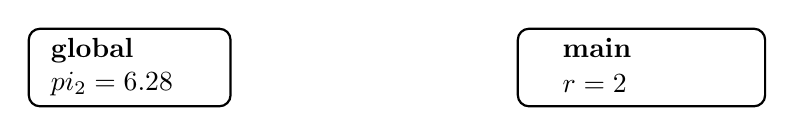
\begin{tikzpicture} [->, >= stealth']
	 	
	 	\node[state] (global)
		 	{

				\begin{tabular}{l}
					\textbf{global} \\
					\parbox{2cm}{
							$pi_2 = 6.28$}
				\end{tabular}
			};

		\node[state, text width=3cm, right of=global, node distance=6.5cm, anchor=center] (main)
			{	\begin{tabular}{l}
					\textbf{main} \\
					\parbox{2cm}{$r=2$}
					
				\end{tabular}
				
			};
%
%	 	
%	 	
%	 	
	 	\end{tikzpicture}
	 	
	 	\subsection{Referenzen}
	 	
	 	\begin{itemize}
	 		\item sind neue (zusätzliche) Namen für vorhandene Speicherzellen
	 		
	 		\begin{lstlisting} [tabsize = 2]
		 		int x = 3;   // neue Variable x mit neuer Speicherzelle
		 		int & y = x; // Referenz: y ist neuer Name fuer x, beide haben dieselbe Speicherzelle
		 		
		 		y = 4; // Zuweisung an y, aber x aendert sich auch, d.h. x == 4
		 		x = 5; // jetzt y == 5
		 		
		 		int const & z = x; // read-only Referenz, d.h. z = 6 ist verboten
		 		x = 6;   // jetzt auch z == 6
	 		\end{lstlisting}
	 		\item Hauptanwendung:
	 		\begin{itemize}
	 			\item Umgebung, wo eine Funktion aufgerufen wird und die Umgebung der Implementation sind unabhängig, d.h. Variablen der einen Umgebung sind in der anderen nicht sichtbar
	 		\end{itemize}
	 		Beispiel: 
	 		\begin{lstlisting} [tabsize = 2]
		 		int foo (int x) {  // pass-by-value (Uebergabe des echten Werts)
			 		x += 3;
			 		return x;
		 		}
		 		
		 		int bar (int & x) {  // pass-by-reference (Uebergabe der Adresse der Speicherzelle)
			 		y += 3;
			 		return y;
		 		}
		 		
		 		void baz (int & z) {  // pass-by-reference
			 		z += 3;  // kein return Wert
		 		}
		 		
			 	int main() {
			 		int a = 2;
			 		std::cout << foo(a) << "\n";  // Ausgabe: 5
			 		std::cout << a << "\n";    // Ausgabe 2
			 		
			 		std::cout << bar(a) << "\n";  // Ausgabe: 5
			 		std::cout << a << "\n";   // Ausgabe: 5
			 		
			 		baz(a);
			 		std::cout << a << "\n";
		 		}
		 		
	 		\end{lstlisting}
	 		\item Funktionen die Werte nur über eine Referenz änder heißen Seiteneffekt der Funktion \\
	 		(Haupteffekt ist immer der return Wert) [in der funktionalen Programmierung sind Seiteneffekte verboten mit Ausnahme von Ein-/Ausgabe]

	 	\item Ziele
	 	\begin{enumerate}
	 		\item häufig möchte man Speicherzellen in beiden Umgebungen teilen $\Rightarrow$ verwende Referenzen
	 		\item häufig will man vermeiden, dass eine Variable kopiert wird (pass-by-value) \\
	 		$\Rightarrow$ durch \textit{pass-by-value} braucht man keine Kopie $\Rightarrow$ typisch $const \, \& \approxeq$ read-only, \underline{keine} Seiteneffekte
	 	\end{enumerate}
	 	
	 	\begin{lstlisting} [tabsize = 2]
	 		void print_string(std::string const & s) {
		 		std::cout << s;
	 		}
	 	\end{lstlisting}
	 \end{itemize}
	 
	 \section{Container-Datentypen}
	 dienen dazu, andere Datentypen aufzubewahren
	 \begin{itemize}
	 	\item Art der Elemente
	 	\begin{itemize}
		 	\item homogene Container: alle Elemente haben den gleichen Typ (typisch für $C++$)
		 	\item heterogene Container: Elemnte können verschiedene Typen haben (z.B. Python)
	 	\end{itemize}
	 	\item Art der Größe
	 	\begin{itemize}
	 		\item statische Container: feste Größe, zur Compilezeit bekannt
	 		\item dynamische Container: Größe zur Laufzeit veränderbar
	 	\end{itemize}
	 	\item Arrays sind die wichtigsten Container, weil effizient auf Hardware abgebildet und einfach zu benutzen
	 	\begin{itemize}
	 		\item klassisch: Arrays sind statisch, z.B. C-Arrays (hat $C++$ geerbt)
	 		\item modern: dynamische Arrays:
	 		\begin{itemize}
	 			\item Entdeckung einer effizienten Implementierung
	 			\item Kapselung durch Objekt-Orientierte-Programmierung (sonst zu kompliziert)
	 		\end{itemize}
	 	\end{itemize}
	 	\item ein dynamisches Array: $std::string$ ist Abbildung $int \rightarrowtail char \quad Index \rightarrow Zeichen$
	 	\item wir wollen das selbe Verhalten für \underline{beliebige} Elementtypen: $std::vector$
	 \end{itemize}
	 	
	 	\paragraph{Datentyp: $std::vector$}
	 	
	 	\begin{itemize}
	 	\begin{lstlisting} [tabsize = 2]
	 		#include <vector>
	 		
	 		std::vector <double> v(20, 0.0) ;  // initialisiert mit Groesse, Initialwert
	 		
	 		// analog: std::vector<int>, std::vector<std::string>
	 	\end{lstlisting}
	 	\item Abbildung: $int \rightarrowtail double$
	 	
	 	\item weitere Verallgemeinerung: Indextyp beliebig (man sagt dann "'Schlüssel-Typ§"' \\
	 	typische Fallen:
	 	\begin{itemize}
	 		\item Index ist nicht im Bereich $0 \leq Index < size$ ,z.B. Matrikelnummer
	 		\item Index ist String, z.B. Name eines Studenten
	 	\end{itemize}
	 	\item $std::map, \, std::unordered_map$ (Binärer Suchbaum) \\ \\
	 	 Beispiel:
	 	 \begin{lstlisting} [tabsize = 2]
	 	 	std::map <int, double> noten;  // noten[3 1 2 4 5  2 3 1 3] = 1.0
	 	 	std::map <string, double> noten;  // noten["krause] = 1.0
	 	 \end{lstlisting}
	 	 dabei: <Schlüsseltyp, Elementtyp>
	 \end{itemize}
	 
	 \begin{itemize}
	 	\item Erzeugen:
	 	\begin{lstlisting} [tabsize = 2]
	 		std::vector <double> v(20, 1.0);
	 		std::vector <double> v;   // leeres Array (erst ab C++ 11)
	 		
	 		std::vector <double> v = {1.0, -3.0, 2.2};  // "initializer list"
	 	\end{lstlisting}
	 	\item Größe:
	 	\begin{lstlisting} [tabsize = 2]
	 		v.size()
	 		v.empty()  (=v.size() ==0)
	 	\end{lstlisting}
	 	\item Größe ändern:
	 	\begin{lstlisting} [tabsize = 2]
	 		v.resize(neue_groesse, initialwert)
			 	1.: neue_gr < size()  // Elemente ab neue_gr geloescht, andere bleiben
			 	2.: neue_gr > size()  // neue Elemente mit Initialwert am Ende angehaengt
			 	
	 		v.push_back(neues_element)  // ein neues Element am Ende anhaengen
	 		
	 		v.insert(v.begin+index, neues_element); // neues Element an Position
								 		// index einfuegen folgende Werte werden 
								 		// um eine Position verschoben
				 	v.begin() ist Iterator
		 	
		 	v.pop_back()  // letztes Element loeschen (effizient)
		 	
		 	v.erase(v.begin()+index)  // Element aus Position loeschen, 
										 	// hintere Werte verschieben
		 	
		 	v.clear()  // alles loeschen
	 	\end{lstlisting}
	 	\item Zugriff:
	 	\begin{lstlisting} [tabsize = 2]
	 		v[k]  // Element bei Index k
	 		v.front()  // erstes Element
	 		v.back()  // letztes Element
	 		
	 		v.at(k)  // wie v[k], aber Fehlermeldung, wenn nicht 0<= k < size()
	 	\end{lstlisting}
	 	\item Funktionen für Container: benutzen in $C++$ Iteration, damit sie für verschiedenste Container funktionieren
	 	\item Iteration-Range: 
	 	\begin{lstlisting} [tabsize = 2]
	 		v.begin()
	 		v.end()  // hinter dem letzten Element
	 		
	 		im Header <algorithm>
	 	\end{lstlisting}
	 	\item alle Elemente kopieren:
	 	\begin{lstlisting} [tabsize = 2]
	 		std::vector <double> source = {1.0, 2.0, 3.0, 4.0, 5.0};
	 		std::vector <double> target(source.size(), 0.0);
	 		
	 		std::copy(source.begin(), source.end(), target.begin());
	 		std::copy(source.begin()+2, source.end(), target.begin());  
			 		// unbenutzte Initialwerte bleiben erhalten
	 	\end{lstlisting}
	 	\item Elemente sortieren:
	 	\begin{lstlisting} [tabsize = 2]
	 		std::sort(v.begin(), v.end());  // "in-place"
	 		std::random_shuffle(v.begin(), v.end())  // "in-place"
	 	\end{lstlisting}
	 \end{itemize}
	 
	 \paragraph{Warum ist $push\_back()$ effizient?}
	 
	 \begin{itemize}
	 	\item veraltete Lehrmeinung: Arrays sind nur effizient, weenn statisch (d.h. Größe zur Compilezeit, spätestens bei Initialisierung bekannt)
	 	\item modern: bei vielen Anwenduungen genügt, wenn Array (meist) nur am Ende vergrößert wird (z.B. $push\_back$) \\
	 	dies kann sehr effizient unterstützt werden $\Rightarrow$ dynamisches Array
	 	\item $std::vector$ verwaltet intern ein statisches Array der Größe "'$v.capacity() >= v.size()$"'
	 	\begin{itemize}
	 		\item wird das interne Array zu klein $\Rightarrow$ wird automatisch auf ein doppelt so großes umgeschaltet
	 		\item ist das interne Array zu groß, bleiben unbenutzte Speicherzellen als Reserve
	 	\end{itemize}
	 	\item Verhalten bei $push\_back()$
	 	\begin{itemize}
	 		\item noch Reserve vorhanden: lege neues Element in eine unbenutzte Speicherzelle $\Rightarrow$ billig \& chillig
	 		\item keine Reserve: 
	 		\begin{enumerate}
	 			\item alloziere neues statisches Array mit doppelter Kapazität
	 			\item kopiere die Daten aus allem ins neue Array
	 			\item gebe das alte Array frei
	 			\item gehe zu  \kreis{1}, jetzt wieder Reserve vorhanden \\ Umkopieren ist nicht teuer, da es nur selten nötig ist
	 		\end{enumerate}
	 		\item Beispiel:
	 		\begin{lstlisting}[tabsize = 2]
	 			std::vector <int> v;
	 			for (int k = 0; k < 32; ++k) {
		 			v.push_back(k);
	 			}
	 		\end{lstlisting}
	 		\begin{tabular} {c|c|c|c|c|c}
		 		k & $cap\, vor \, p\_b()$ & $cap\, nach \, p\_b()$ & $size()$ & Reserve & Umkopierung \\
		 		\hline
		 		0 & 0 & 1 & 1 & 0 & 0 \\
		 		1 & 1 & 2 & 2 & 0 & 1 \\
		 		2 & 2 & 4 & 3 & 1 & 2 \\
		 		3 & 4 & 4 & 4 & 0 & 0 \\
		 		4 & 4 & 8 & 5 & 3 & 4 \\
		 		5 $\dots$ 7 & 8 & 8 & 8 & 0 & 0 \\
		 		8 & 8 & 16 & 9 & 7 & 8 \\
		 		9 $\dots$15 & 16 & 16 & 16 & 0 & 0 \\
		 		16 & 16 & 32 & 17 & 15 & 16 \\
	 		\end{tabular} \\ \\
	 				 		$\cdots$
	 	\end{itemize}
	 	
	 	\item Kosten:
	 	\begin{itemize}
	 		\item 32 Elemente einfügen $=$ 32 Kopien extern $\Rightarrow$ intern
	 		\item aus altem Array ins neue kopieren $=$ 31 Kopien intern $\Rightarrow$ intern \\
	 		$\Rightarrow$ im Durchschnitt sind pro Einführung 2 Kopien nötig \\
	 		$\Rightarrow$ dynamisches Array ist doppelt so teuer, wie das statische \\
	 		$\Rightarrow$ immer noch sehr effizient
	 	\end{itemize}
	 	\item relevante Funktionen von $std::vector$
	 	\begin{itemize}
	 		\item $v.size()$: aktuelle Zahl der Elemente
	 		\item $v.capacity()-v.size()$: Reserve ($\geq 0$)
		 	\item $v.resize(new\_size)$: ändert immer $v.size()$, aber $v.capacity()$ nur wenn $< new\_size$
		 	\item $v.reserve(new\_capacity)$: ändert $v.size()$ nicht, aber $v.capacity()$ falls $new\_capacity \geq size$
		 	\item $v.shrink\_to\_fit()$: $v.reserve(v.size())$ (Reserve ist danach 0), wenn Endgröße erreicht
	 	\end{itemize}
	 	\item wenn Reserve $> size$: $capacity$ kann auch halbiert werden
	 \end{itemize}
	 
	 \paragraph{wichtige Container der $C++$ Standardbiblithek}
	 
	 \begin{itemize}
	 	\item dynamisches Arrays: $std::string, std::vector$
	 	\item assoziative Arrays: $std::map, std::unordered\_map$
	 	\item Mengen: $std::set, std::unordered\_set$ (jedes Element ist höchstens einmal enthalten)
	 	\item Stapel: $std::stack$ (Funktion: "'last-in-first-out"') z.B. gestapelte Bierkästen.
	 	\item Warteschlange: $std::queue$ (Funktion: "'first-in-first-out"')
	 	\item Kartendeck: $std::deque$ gleichzeitig Stapel und Warteschlange
	 	\item Stapel mit Priorität: $std::priority\_queue$ (Priorität vom Nutzer definiert)
	 \end{itemize}
	 	
	 \section{Iteratoren}
	\begin{itemize}
		\item für Arrays lautet kanonische Schleife:
		\begin{lstlisting} [tabsize = 2]
			for (int k = 0; k != v.size(); ++k) {
				int current = v[k];  // aktuelles Element lesen
				v[k] = new_value;  // aktuelles Element schreiben
			}
		\end{lstlisting}
		\item wir wollen eine so einfache Schleife für beliebige Container
		\begin{itemize}
			\item der Index-Zugriff $v[k]$ ist bei den meisten Containern nicht effizient
			\item Iteratoren sind immer effizient $\Rightarrow$ es gibt sie in allen modernen Programmiersprachen, aber die Details sind sehr unterschiedlich
			\item Analogie: Zeiger einer Uhr, Cursor in Textverarbeitung \\
			$\Rightarrow$ ein Iterator zeigt immer auf ein Element des Containers oder auf Spezialwert "'ungültiges Element"'
			\item in $C++$ unterstützt jeder Iterator 5 Grundoperationen
			\begin{enumerate}
				\item Iterator auf erstes Element erzeugen:
				\begin{lstlisting} [tabsize = 2]
					auto iter = v.begin();  // auto ist Universaltyp, wird 
													// vom Compiler automatisch
													//  mit richtigen Typen ersetzt
				\end{lstlisting}
				\item Iterator auf "'ungültiges Element"' erzeugen:
				\begin{lstlisting} [tabsize = 2]
					auto end = v.end()  // typischerweise v[v.size()]
				\end{lstlisting}
				\item Vergleich:
				\begin{lstlisting} [tabsize = 2]
					iter1 == iter2;
					iter != end;  (= !(iter == end))  // iter zeigt nicht auf
																  // ungueltiges Element
				\end{lstlisting}
				\item zum nächsten weitergehen: $++iter$, Ergebnis ist $v.end()$, wenn man vorher beim letzten Element war
				\item auf Daten des aktuellen Elements zugreifen: $*iter$ ("'Dereferenzierung"')
			\end{enumerate}
		\end{itemize}
		\item $\Rightarrow$ kanonische Schleife:
		\begin{lstlisting} [tabsize = 2]
			for (auto iter = v.begin(); iter != v.end(); ++iter) {
				int current = *iter;  // lesender Zugriff;
				*iter = new_value;  // schreibender Zugriff
				
				// Abkuerzung in C++: rang-based for-loop
				for (int & element : v) {
					int current = element;  // lesen
					element = new_value;  // schreiben
				}
			}
		\end{lstlisting}
		\item wenn die zugrunde liegenden Speicherzellen geändert werden, also die Containergröße sich ändert, werden die Iteratoren ungültig
		\item Iteratoren mit den 5 Grundoperationen heißen "'forward iterators"' (wegen $++iter$)
		\item "'bidirectional iterators"' unterstützen auch $--iter$ (alle Iteratoren aus Standardbibliothek)
		\item "'random access iterators"' können beliebige Sprünge machen ($iter+=5$) \\
		unterstützt von $std::string$ und $std::vector$
		\item Besonderheit für assoziative Arrays ($std::map$):
		\begin{itemize}
			\item Schlüssel und Werte können beliebig gewählt werden \\
			$\Rightarrow$ das aktuelle Element ist immer ein Schlüssel/Wert-Paar \\
			$(*iter).first \Rightarrow$ Schlüssel \\
			$(*iter).second \Rightarrow$ Wert
			\begin{lstlisting} [tabsize = 2]
				v[(*iter).first] == (*iter).second;
			\end{lstlisting}
		\end{itemize}
		\item Bei $std::map$ liefern die Iteratoren die Elemente in aufsteigender Reihenfolge der Schlüssel (Unterschied zu $std::unordered\_map$)
	\end{itemize}
	
	\subsection{Die Funktion $std::transform()$}

	\paragraph{Die Funktion $std::transform()$}
	
	\begin{itemize}
		\item $std::transform()$ erlaubt, die Daten "'on-the-fly"' zu ändern \\
		z.B. nach Kleinbuchstaben konvertieren:
		\begin{lstlisting} [tabsize = 2]
			std::string source = "aAbCdE";std::string = target = source;  // Target muss gleiche Laenge haben
			std::transform(source.begin(), source.end(), target.begin(), std::tolower); //Name einer Funktion, die ein einzelnes Element transformiert
		\end{lstlisting}
		
		\item z.B. die Daten quadrieren:
		\begin{lstlisting} [tabsize = 2]
			double sq (double x) {
				return x*x;
			}
			
			std::transform(source.begin(), source.end(), target.begin(), sg);
		\end{lstlisting}
		
		\item das ist eine Abkürzung für eine Schleife: (zwei Schleifen auf einmal)
		\begin{lstlisting} [tabsize = 2]
			auto src_begin = source.begin();
			auto src_end = source.end();
			auto tgt_begin = target.begin();
			
			for ( ; src_begin != src_end; ++src_begin, ++tgt_begin) {  
							// mehrere Inkrementierungen durch , getrennt
				*tgt_begin = sq(*src_begin);  // mit * Bezug zu originalen Daten
			}
		\end{lstlisting}
		
		\item der Argumenttyp der Funktion muss mit dem $source$-Elementtyp kompatibel sein
		\item der Argumenttyp der Funktion muss mit dem $target$-Elementtyp kompatibel sein
	
	\item Das letzte Argument von $std::transform()$ muss ein Funktor sein ($\approxeq$ verhält sich wie eine Funktion) \\
	Dazu gibt es drei Varianten:
		\begin{enumerate}
			\item normale Funktion, z.B. $sq$ Aber wenn die Funktion für mehrere Argumenttypen überladen ist, muss der Programmierer dem Compiler sagen, welche Version gemeint ist \\ $\Rightarrow$ ("'function pointer cast"')
			\item  Funktorobjekte $\Rightarrow$ objekt-orientierte Programmierung
			\item definiere eine namenlose Funktion $\approxeq$"'Lamda-Funktionen"' $\lambda$ \\
			statt $\lambda$ wird in $C++$ $[]$ geschrieben
		\end{enumerate}
		\begin{lstlisting} 	[tabsize = 2]
			std::transform(source.begin(), source.end(), target.begin(), 
				[] (double x) {  // statt Funktionsname sq, wie bei 1. 
									// steht hier die ganze Funktionsimplementierung
					return x*x
				});  // der Returntypwird automatisch eingesetzt, wenn es 
					 // nur einen Returntyp gibt
		\end{lstlisting}
		\begin{itemize}
			\item Lambda-Funktionen können noch viel mehr $\Rightarrow$ für Fortgeschrittene
			\item $std::transform$ kann "'in-place"' arbeiten (d.h. source-Container überschreiben), wenn source und target gleich
			\item die Funktion $std::sort()$ wird zum "'in-place"' sortieren eines Arrays
			\begin{lstlisting} [tabsize = 2]
				std::vector <double> v = {4.0, 2.0, 3.0, 5.0, 1.0};
				std::sort(v.begin(), v.end());  // -> v = {1.0, 2.0, 3.0, 4.0, 5.0}
			\end{lstlisting}
			
			\item $std::sort()$ ruft intern den "'<"' Operator des Elementtyps auf, um die Reihenfolge zu bestimmen \\ \\
			\underline{Def:} "'totale Ordnung"'
			\begin{itemize}
				\item $a<b$ muss $\forall a,b$ gelten
				\item transitiv: ($a<b$) $\wedge$ ($b<c$) $\Rightarrow$ ($a<c$)
				\item anti-symmetrisch: $!(a<b) \wedge !(b<a) \Rightarrow a ==b$
			\end{itemize}
		\end{itemize}
	\end{itemize}
	
	\subsection{Insertion Sort}
	schnellste Sortieralgor. für kleine Arrays ($n\leq 30$, hängt vom Compiler \& CPU ab)
	\begin{itemize}
		\item für große Arrays sind Merge Sort, Heap Sort, Quick Sort schneller
		\item $std::sort()$ wählt automatisch einen schnellen Algor.
	\end{itemize}
	
	Idee von Insertion Sort: wie beim Aufnehmen und Ordnen eines Kartenblatts
	\begin{itemize}
		\item gegeben: bereits sortiertes Teilarray bis zur Position $k-1$
		\item füge das k-te Element an der richtigen Stelle ein. Erzeuge Lücke an der richtigen Position duch Verschieben von Elementen nach rechts
		\item wiederhole für $k = 1,\dots , N$  (siehe Übung 5.1 "'Einsortieren"')
	\end{itemize}
	\begin{tabular} {cccccc}
		4 & 2 & 3 & 5 & 1 & \\  
		4 & & 3 & 5 & 1 & (current = 2) \\
		 & 4 & 3 & 5 & 1 & \\
		 2 & 4 & 3 & 5 & 1 & \\
		 2 & 4 & & 5 & 1 & (current = 3) \\ 
		 2 & & 4 & 5 & 1 & \\
		 2 & 3 & 4 & 5 & 1 & \\ 
		 2 & 3 & 4 & 5 & 1 & \\	 
		 2 & 3 & 4 &  & 1 & (current = 5)	\\		 
		 2 & 3 & 4 & 5 & 1 & \\		
		 2 & 3 & 4 & 5 & 1 & (current = 1)	\\   
		 1 & 2 & 3 & 4 & 5 & \\
	\end{tabular}
	
	\begin{lstlisting} [tabsize = 2]
		void insertion_sort(std::vector <double> &v) {
			for ( int K = 1; k < v.size(); ++k) {
				double current = v[k];
				int j = k;   // Anfangsposition der Luecke
				while (j>0) {
					if (v[j-1] < current) {
						break;   // j ist richtige Position der Luecke
					}
					v[j] = v[j-1];
					--j;
				}
				v[j] = current;   // current in die Luecke kopieren
			}
		}
	\end{lstlisting}
	\begin{itemize}
		\item andere Sortierung: definiere Funktor $cmp(a,b)$ , der das gewünschte "'kleiner"' realisiert $\approxeq$ gibt genau dann $true$ zurück, wenn $a$ "'kleiner $b$ nach neuer Sortierung
		\item neue Sortierungen am besten per Lambda-Funktion an $std::sort$ übergeben
		\begin{lstlisting}
			std::sort(v.begin(), v.end());  // Standardsortierung aufsteigend
			
			std::sort(v.begin(), v.end(),   // Standardsortierung aufsteigend
							[](double a, double b) {
								return a<b;
							}
			)
			
			std::sort(v.begin(), v.end(),   // absteigende Sortierung
						[](double a, double b) {
							return b<a;
						}
			)
						
			std::sort(v.begin(), v.end(),   //   normale Sortierung nach Betrag
						[](double a, double b) {
							return std::abs(a) < std::abs(b);
						}
			)
			
			// Stringvergleich 
			std::vector <std::string> v = {"Ac", "ab", "De", "cf"};  
			std::vector <std::string> v = {"Ac", "De", "ab", "cf"}  // case insensitive
			std::vector <std::string> v = {"ab", "Ac", "cf", "De"}  // case sensitive
			
		\end{lstlisting}
	\end{itemize}

	\begin{itemize}
	\item Das letzte Argument von $std::transform()$ muss ein Funktor sein ($\approxeq$ verhält sich wie eine Funktion) \\
	Dazu gibt es drei Varianten:
		\begin{enumerate}
			\item normale Funktion, z.B. $sq$ Aber wenn die Funktion für mehrere Argumenttypen überladen ist, muss der Programmierer dem Compiler sagen, welche Version gemeint ist \\ $\Rightarrow$ ("'function pointer cast"')
			\item  Funktorobjekte $\Rightarrow$ objekt-orientierte Programmierung
			\item definiere eine namenlose Funktion $\approxeq$"'Lamda-Funktionen"' $\lambda$ \\
			statt $\lambda$ wird in $C++$ $[]$ geschrieben
		\end{enumerate}
		\begin{lstlisting} 	[tabsize = 2]
			std::transform(source.begin(), source.end(), target.begin(), 
				[] (double x) {  // statt Funktionsname sq, wie bei 1. 
									// steht hier die ganze Funktionsimplementierung
					return x*x
				});  // der Returntypwird automatisch eingesetzt, wenn es 
					 // nur einen Returntyp gibt
		\end{lstlisting}
		\begin{itemize}
			\item Lambda-Funktionen können noch viel mehr $\Rightarrow$ für Fortgeschrittene
			\item $std::transform$ kann "'in-place"' arbeiten (d.h. source-Container überschreiben), wenn source und target gleich
			\item die Funktion $std::sort()$ wird zum "'in-place"' sortieren eines Arrays
			\begin{lstlisting} [tabsize = 2]
				std::vector <double> v = {4.0, 2.0, 3.0, 5.0, 1.0};
				std::sort(v.begin(), v.end());  // -> v = {1.0, 2.0, 3.0, 4.0, 5.0}
			\end{lstlisting}
			
			\item $std::sort()$ ruft intern den "'<"' Operator des Elementtyps auf, um die Reihenfolge zu bestimmen \\ \\
			\underline{Def:} "'totale Ordnung"'
			\begin{itemize}
				\item $a<b$ muss $\forall a,b$ gelten
				\item transitiv: ($a<b$) $\wedge$ ($b<c$) $\Rightarrow$ ($a<c$)
				\item anti-symmetrisch: $!(a<b) \wedge !(b<a) \Rightarrow a ==b$
			\end{itemize}
		\end{itemize}
	\end{itemize}
	
	\subsection{Insertion Sort}
	schnellste Sortieralgor. für kleine Arrays ($n\leq 30$, hängt vom Compiler \& CPU ab)
	\begin{itemize}
		\item für große Arrays sind Merge Sort, Heap Sort, Quick Sort schneller
		\item $std::sort()$ wählt automatisch einen schnellen Algor.
	\end{itemize}
	
	Idee von Insertion Sort: wie beim Aufnehmen und Ordnen eines Kartenblatts
	\begin{itemize}
		\item gegeben: bereits sortiertes Teilarray bis zur Position $k-1$
		\item füge das k-te Element an der richtigen Stelle ein. Erzeuge Lücke an der richtigen Position duch Verschieben von Elementen nach rechts
		\item wiederhole für $k = 1,\dots , N$  (siehe Übung 5.1 "'Einsortieren"')
	\end{itemize}
	\begin{tabular} {cccccc}
		4 & 2 & 3 & 5 & 1 & \\  
		4 & & 3 & 5 & 1 & (current = 2) \\
		 & 4 & 3 & 5 & 1 & \\
		 2 & 4 & 3 & 5 & 1 & \\
		 2 & 4 & & 5 & 1 & (current = 3) \\ 
		 2 & & 4 & 5 & 1 & \\
		 2 & 3 & 4 & 5 & 1 & \\ 
		 2 & 3 & 4 & 5 & 1 & \\	 
		 2 & 3 & 4 &  & 1 & (current = 5)	\\		 
		 2 & 3 & 4 & 5 & 1 & \\		
		 2 & 3 & 4 & 5 & 1 & (current = 1)	\\   
		 1 & 2 & 3 & 4 & 5 & \\
	\end{tabular}
	
	\begin{lstlisting} [tabsize = 2]
		void insertion_sort(std::vector <double> &v) {
			for ( int K = 1; k < v.size(); ++k) {
				double current = v[k];
				int j = k;   // Anfangsposition der Luecke
				while (j>0) {
					if (v[j-1] < current) {
						break;   // j ist richtige Position der Luecke
					}
					v[j] = v[j-1];
					--j;
				}
				v[j] = current;   // current in die Luecke kopieren
			}
		}
	\end{lstlisting}
	\begin{itemize}
		\item andere Sortierung: definiere Funktor $cmp(a,b)$ , der das gewünschte "'kleiner"' realisiert $\approxeq$ gibt genau dann $true$ zurück, wenn $a$ "'kleiner $b$ nach neuer Sortierung
		\item neue Sortierungen am besten per Lambda-Funktion an $std::sort$ übergeben
		\begin{lstlisting} [tabsize = 2]
			std::sort(v.begin(), v.end());  // Standardsortierung aufsteigend
			
			std::sort(v.begin(), v.end(),   // Standardsortierung aufsteigend
							[](double a, double b) {
								return a<b;
							}
			)
			
			std::sort(v.begin(), v.end(),   // absteigende Sortierung
						[](double a, double b) {
							return b<a;
						}
			)
						
			std::sort(v.begin(), v.end(),   //   normale Sortierung nach Betrag
						[](double a, double b) {
							return std::abs(a) < std::abs(b);
						}
			)
			
			// Stringvergleich 
			std::vector <std::string> v = {"Ac", "ab", "De", "cf"};  
			std::vector <std::string> v = {"Ac", "De", "ab", "cf"}  // case insensitive
			std::vector <std::string> v = {"ab", "Ac", "cf", "De"}  // case sensitive
			
			std::sort(v.begin(), v.end(), 
						[](std::string a, std::string b) {
							std::transform(a.begin(), a.end(), a.begin(), std::tolower);
							std::transform(b.begin(), b.end(), b.begin(), std::tolower);
							
							retuern a<b;
						}
			);
			
		\end{lstlisting}
	\end{itemize}
	
	\section{Templates}
	$insertion\_sort$ soll für beliebige Elementtypen funktionieren:
	
	\begin{lstlisting} [tabsize = 2]
		template <typename ElementType>
		
		void insertion_sort(std::std::vector <ElementType> & v) {
			for (int k =1; k < v.size(); ++k) {
				ElementType current = v[k];
				...   // Rest unveraendert
			}
		}
	\end{lstlisting}
	
	"'ElementType"' ist Platzhalter für den tatsächlichen Elementtyp und wird vom Compiler automatisch ersetzt.
	
	
	\section{Grundlagen der generischen Programmierung}
	
	\begin{itemize}
		\item Ziel: benutze $template$-Mechanismus, damit \underline{eine} Implementation für viele verschiedene Typen verwendbar ist \\
		erweitert funktionale und prozedurale und objekt-orientierte Programmierung
		\item zwei Arten von Templates ("'Schablonen"')
		\begin{enumerate}
			\item Klassen-Templates für Datenstrukturen, z.B. Containersollen beliebige Elementtypen unterstützen
			\begin{itemize}
				\item Implementation $\Rightarrow$ später
				\item Benutzung: Datenstrukturname gefolgt vom Elementtyp in spitzen Klammern \\
				$std::vector\, <double>$
			\end{itemize}
			\item Funktionen-Templates: es gab schon "'function overloading"' \\
			Beispiel:
			\begin{lstlisting} [tabsize = 2]
				int sq (int x) {
					return x * x;
				}
				
				double sq (double x) {
					return x * x;
				}
				... usw fuer komplexe Zahlen
			\end{lstlisting}
			$\Rightarrow$ Nachteile:
			\begin{itemize}
				\item wenn die Implementationen gleich sind nutzlose Arbeit
				\item Redundanz ist gefährlich, korrigiert man ein Bug, wird leicht eine Variante vergessen
			\end{itemize}
		\end{enumerate}
	\end{itemize}
			
	\subsection{Funktionen-Templates}
			mit Templates reicht eine Implementation:
			\begin{lstlisting} [tabsize = 2]
				template <typename T>  // T ist Platzhalter fuer beliebigen Typ
										// wird spaeter durch einen tatsaelichen Typ ersetzt
				T sq (T x) {
					return x * x;  // impliziete Anforderung an den Typ:
								// er muss Multiplikation unterstuetzen
					
				}
			\end{lstlisting}
	\begin{itemize}
		\item Benutzung:
		\begin{itemize}
			\item Typen für die Platzhalter hinter dem Funktionsnamen in spitzen Klammern
			\item meist kann man die Typangabe $<type>$ weglassen, weil der Compiler sie anhand des Argumenttyps automatisch einsetzt
		\end{itemize}
		\item kombiniert man Templates mit Overloading, wird die ausprogrammierte Variante vom Compiler bevorzugt
		\item Funktion, die ein Array aus Konsole ausgibt:
		\begin{lstlisting} [tabsize = 2]
			std::vector <double> v = {1.0, 2.0, 3.0};
			print_vector(v);  // {1.0, 2.0, 3.0}
		\end{lstlisting}
		für beliebige Elementtypen:
		\begin{lstlisting} [tabsize = 2]
			template <typename ElemtType>
			void print_vector(std::vector <ElementType> const & v) {
			// const: read-only , &: nur Kopie verwenden
				std::cout << "{";
				if ( v.size() > 0) {
					std::cout << " " << v[0];
					for (int k = 1; k<v.size(); ++k) {
						std::cout <<  " " << v[k];
					}
				}
				std::cout << " }";
			}
		\end{lstlisting}
		\item Verallgemeinerung für beliebige Container mittels Iteratoren:
		\begin{lstlisting}
			std::list <int> l = {1,2,3};
			print_container (l.begin(), l.end())  // {1,2,3}
		\end{lstlisting}
		\item es genügen forward iterators
		\begin{lstlisting} [tabsize = 2]
			Iterator iter2 = iter;  // Kopie erzeugen
			++iter1;  // zum naechsten Element
			iter1 == iter2, iter1 != end  // zeigen sie auf das selbe Element
			+ iter1  // Zugriff auf aktuelles Element
			
			template <typename Iterator>
			
			void print_container(Iterator begin, Iterator end) {
				std::cout << "{";
				if (begin != end) {  // teste, ob Container leer
					std::cout << " " << *begin;
					++begin;
					for (; begin != end; ++begin) {
						std::cout << ", " << *begin;
					}
				}
				std::cout << "}";
			}
		\end{lstlisting}
		\item Beispiel 3: checken, ob Container sortiert ist
		\begin{lstlisting} [tabsize = 2]
			Version 1: hard-coded
			
			bool check_sorted (std::vector <double> const & v) {
				for (int k = 1; k < v.size(); ++k) {
					if (v[k] < v[k-1]) {  // Sortierfehler durch Ausnutzen 
												 // der Transitivitaet
							return false;
					}
				}
				return true;  // Schleife ohne Fehler zuende gelaufen
			}
			
			Version 2: beliebige Elementtypen, beliebige Sortierung
			
			template <typename ElementType, typename LessThanFunctor>
			
			bool check_sorted(std::vector<ElementType> const & v, typename LessThanFunctor) {
				for (int k = 1; k < v.size(); ++k) {
					if (less_than(v[k], v[k-1])) {
						return false;
					}
				}
				reurn true;
			}
		\end{lstlisting}
		\begin{itemize}
			\item Aufruf von Version 2 mit "'lambda-function"':
			\begin{lstlisting}
				std::vector <double> v = {1.0, 2.0, 3.0};
				check_sorted(v, [] (double a, double b) {
					return a<b;
				});  // true
				
				check_sorted(v, [] (double a, double b) {
					return a>b;
				});  // true
			\end{lstlisting}
			\item Version 3 mit "'forward-iterator"':
			\begin{lstlisting}
				template <typename Iterator, typename LessThanFunctor>
				bool check_sorted(Iterator begin, Iterator end, 
								LessThanFunctor less_than)
					{
						if (begin == end) {  // Container leer?
							return true;  // leerer Container immer sortiert
						}
						Iterator next = begin;  
						++ next;  // next zeigt auf Element nach Iterator begin
						
						for (; next != end; ++begin, ++next) {  // Iteratoren zeigen 
														//auf zwei benachbarte Elemente
							if (less_than(*next , *begin))	{
								return false;
							}
						}
					}
			\end{lstlisting}
		\end{itemize}
		\item Bemerkungen:
		\begin{enumerate}
			\item Compiler-Fehlermeldungen bei Template-Code sind oft schwer zu implementieren $\Rightarrow$ Erfahrung nötig
			\item mit Templates kann man noch viel raffiniertere Dinge machen, z.B. Traits-Klassen, intelligent libraries, template metaprogramming $\Rightarrow$ nur für Fortgeschrittene
		\end{enumerate}
	\end{itemize}
	
	\section{Bestimmung der Effizienz von Algorithmen und Datenstrukturen}
	
	\begin{itemize}
		\item 2 Möglichkeiten
		\begin{enumerate}
			\item messe die "'wall clock time"' (wie lange muss man auf ein Ergebnis warten)
			\item unabhängig von Hardware: algorithmische Komplexität
		\end{enumerate}
		\item "'wall-clock-time"' misst man z.B. mit dem Modul $<chrono>$
		\begin{lstlisting}
			#include <chrono>
			#include <iostream>
			
			int main() {
				...  // alles zur Zeitmesung vorbereiten, z.B. Daten einlesen
				
				auto start = std::chrono::high_resolution_clock::now();  // Startzeit merken
					...  // Code, der gemessen werden soll
				auto stop = std::chrono::high_resolution_clock::now();  // Endzeit merken
				std::chrono::duration<double> diff = stop-start;  // Zeitdifferenz (Laufzeit) in Sekunden
				std::cout << "Zeitdauer: " << diff() << " sekunden \n";)
			}
		\end{lstlisting}
		\item in der Praxis nicht so einfach $\Rightarrow$ Pitfalls:
		\begin{itemize}
			\item moderne Compiler optimieren oft zu viel, d.h. komplexe Berechnungen werden zur Compilezeit ausgeführt und ersetzt $\Rightarrow$ gemessene Zeit viel zu kurz gegenüber der Praxis \\
			Abhilfe: Daten nicht "'hard-wired"', sondern z.B. von Platte lesen ($volatile$ beim Initialisieren)
			\item der Algorithmus ist schneller als die clock  \\
			Abhilfe: rufe den Algorithmus mehrmals in einer Schleife auf
		\item die Ausstattung des Programms kann vom Betriebssystem jederzeit für etwas wichtigeres unterbrochen werden $\Rightarrow$ gemessene Zeit ist zu lang \\
		Abhilfe: messe mehrmals und nimm die kürzeste Zeit (meist reicht 3-10x)
		\item Faustregel: Messung zwischen 0.02-3 Sekunden zur optimalen Nutzung der clock
		\end{itemize}
		\item Nachteil: Zeit hängt besonders von der Qualität der Implementation, den Daten und der Hardware ab
		\item algorithmische Komplexität ist davon unabhängig $\approxeq$ "'theoretisches Effizienzmaß"' \\
		beschreibt, wie sich die Laufzeit verlängert, wenn man mehr Daten hat \\
		
		$\Rightarrow$ bei effizienten Algrorithmen steigt der Aufwand mit n nur langsam (oder bestenfalls gar nicht)
		
		\subsection{technisches Effizienzmaß}
		\begin{itemize}
			\item berechne, wie viele elementare Schritte der Algorithmus in Abhängigkeit von n benötigt $\Rightarrow$ komplizierte Formel $f(n)$
			\item vereinfache $f(n)$ in eine einfache Formel $g(n)$, die dasselbe wesentliche Verhalten zeigt  \\
			Die Vereinfachung erfolgt mittels \underline{O-Notation} und ihren Verwandten
		\end{itemize}
		
		\subsection{$\mathcal{O}$-Notation/$\Omega$-Notation}
		\begin{enumerate}
			\item $g(n)$ ist eine asymptotische (für große n) obere Schranke für $f(n)$ ($f(n) \leq g(n)$) \\
			$f(n) \in \mathcal{O}(g(n))$ ($f(n)$ ist in der Komplexitätsklasse $g(n)$, wenn es ein $n_0$ und $C$ gibt, sodass $\forall n > n_0: \Leftrightarrow f(n) \in \mathcal{O}(g(n))$
			
			\item $g(n)$ ist asymptotisch untere Schranke für $f(n)$ ($f(n) \geq g(n)$) \\
			$f(n) \in \Omega(g(n)) \Leftrightarrow \exists n_0, C , sodass\, \forall n>n_0: f(n) \geq C \cdot g(n)$
			\item $g(n)$ ist  asymptotisch scharfe Schranke für $f(n)$ ($f(n) = g(n)$) \\
			$f(n) \in \Theta(g(n)) \Leftrightarrow f(n) \in O(g(n)) \wedge f(n) \in \Omega(g(n))$
		\end{enumerate}
		Regeln:
		\begin{enumerate}
			\item $f(n) \in \Theta(f(n)) \Rightarrow f(n) \in \mathcal{O}(f(n)), f(n) \in \Omega/f(n))$
			\item $f(n) \in \Theta(f(n)) \Rightarrow C \cdot f(n) \in \Theta(f(n))$
			\item $\mathcal{O}(f(n)) \cdot \mathcal{O}(g(n)) \in = \mathcal{O}(f(n) \cdot g(n))$
			\item $O(f(n)) + O(g(n)) \in O(max(f(n),g(n))$ \\
			formell: $f(n) \in O(g(n)) \Rightarrow O(f(n)) + O(g(n)) \in O(g(n))$
						$g(n) \in O(f(n)) \Rightarrow O(g(n)) + O(g(n)) \in O(f(n))$
			
		\end{enumerate}
		\begin{itemize}
			\item beliebteste Wahl für $g(n)$:
			\begin{itemize}
				\item $\mathcal{O}(1)$ "' konstante Komplexität"', Bsp: elementare Operationen, Array-Zugriff
				\item $\mathcal{O}(log(n))$ "'logarithmische Komplexität"', Bsp: Zugriff auf ein Element von $std::map$
				\item $\mathcal{O}(n)$ "'lineare Komplexität"', Bsp: $std::transform$
				\item $\mathcal{O}(log(n) \cdot n)$ "'$n \cdot log(n)$"',"'quasilinear"', Bsp: $std::sort()$
				\item $\mathcal{O}(n^2)$ "'quadratische Komplexität"'
				\item $\mathcal{O}(n^p) p=const.$ "'polynomelle Komplexität"'
				\item $\mathcal{O}(2^n)$ "'exponentielle Komplexität"'
			\end{itemize}
			\item Beispiele:  \\
			$f(n)=1+15n+4n^2+7n^3 \in \mathcal{O}(n^3)$ \\
			$f(n)=n \cdot log(n) + n^2 \in \mathcal{O}(n \cdot log(n) + n\cdot n) \in \mathcal{O}(n) \cdot \mathcal{O}(log(n) + n) \in \mathcal{O}(n) \cdot \mathcal{O}(n) \in \mathcal{O}(n^2)$
			
			$\Rightarrow$ es gewinnt immer die am stärksten wachsende Funktion
		\end{itemize}
		Anwendung 1: Fibonacci-Zahlen: $f_k = f_{k-2} + f_{k-1}$  \\ \\
		\begin{tabular} {c|c|c|c|c|c|c|c|c|c}
			k & 0 & 1 & 2 & 3 & 4 & 5 & 6 & 7 & 8 \\
			\hline
			$f_k$ & 0 & 1 & 1 & 2 & 3 & 5 & 8 & 13 & 21 
		\end{tabular} \\
		\begin{lstlisting}
			int fib1 (int k) {  // O(k)
				if (k<2) {  // O(1)
					return k;  // O(1)
				}
				int f1 = 1;  // O(1)
				int f2 = 1;  // O(1)
			
				for (int j = 2; j<=k; ++j) {  // O(k)
					int f = f1 + f2;  // O(1)
					f1 = f2;  // O(1)
					f2 = f;  // O(1)
				}
				
				return f2;  // O(1)
			}
			
			int fib2 (int k) {
				if (k<2) {
					return k;
				}
				return fib2(k-2)+fib2(k-1));
			}
		\end{lstlisting}
		
		 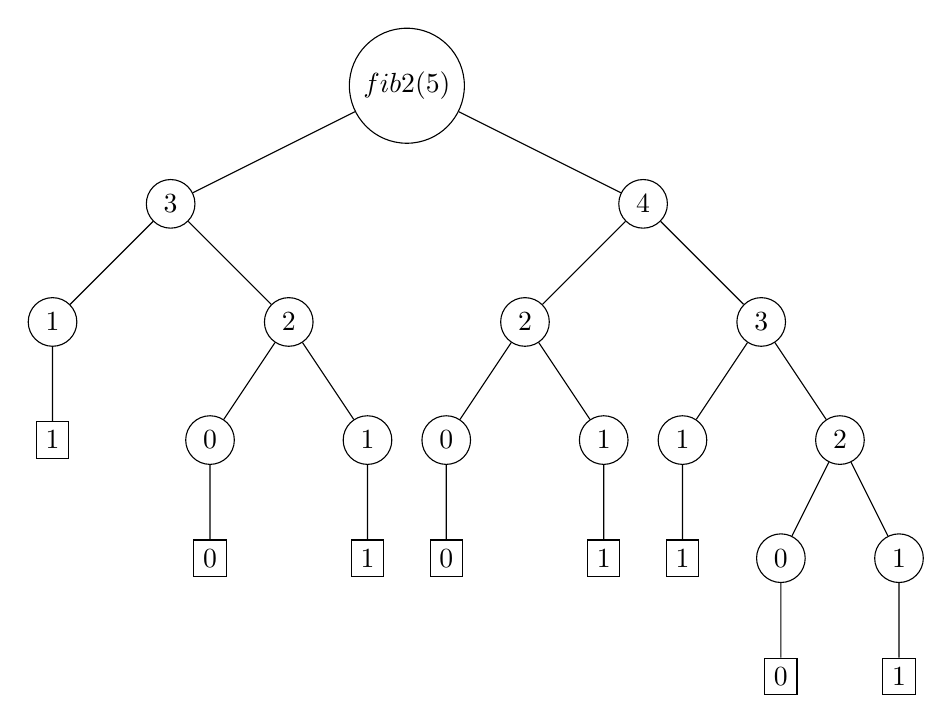
\begin{tikzpicture}[level/.style={sibling distance=60mm/#1}]
		 
		 \node [circle, draw] (z)  {$fib2(5)$}
		 child {node [circle, draw] {$3$}
		 	child {node [circle, draw] {$1$}
		 		child{node [draw] {$1$}}
		 	}
		 	child {node [circle, draw] {$2$}
		 		child{node [circle, draw] {$0$}
		 			child {node [draw] {$0$}}
		 		}
		 		child{node [circle, draw] {$1$}
		 			child {node [draw] {$1$}}
		 		}
		 	}}
		 	child {node [circle, draw] {$4$}
		 		child{node [circle, draw] {$2$}
			 		child{node [circle, draw] {$0$}
				 		child{node [draw] {$0$}}
				 	}
				 	child{node [circle, draw] {$1$}
					 	child{node [draw] {$1$}}
					}}
				 child{node [circle, draw] {$3$}
					child{node [circle, draw] {$1$}
						  child{node [draw] {$1$}}
					 }
					 child {node [circle, draw] {$2$}
					 	child{node [circle, draw] {$0$}
					 		child {node [draw] {$0$}}
					 	}
					 	child{node [circle, draw] {$1$}
					 		child {node [draw] {$1$}}
					 	}
					 }}
		 	};
		 	\end{tikzpicture} \\
		$\Rightarrow$ sehr ineffizient, weil alle Fib-Zahlen $<k$ mehrmals berechnet werden \\
		Sei $f(k)$ die Anzahl der Schritte, Annahme: jeder Knoten ist $\mathcal{O}(1) \Rightarrow \mathcal{O}(Knoten)$
		Sei $f'(k)$ die Anzahl der Schritte, oberhalb (oberhalb ist der Baum vollständig (jeder innere Knoten hat genau 2 Kinder))
		\begin{align*}
			 f'(k) &= 2^{l+1}-1 \\
			 &= 2^{k/2+1}-1 \\
			 &= 2 \cdot 2^{k/2}-1 \\
			 &= 2 \cdot (\sqrt{2})^k-1 \\ &\in \Omega(\sqrt{2})^k  \\
			 & \Rightarrow exponentielle \, Komplexit\ddot{a}t \\
		\end{align*}
	\end{itemize}
	
\section{Zahlendarstellung}
	Problem: unendlich viele Zahlen, aber die Computer sind endlich
\subsection{natürliche Zahlen $\mathbb{N}$}
	$x \geq 0$, ($++$ bietet Typen verschiedener Größe) \\

	\begin{tabular} {c|c|c|c|c}
		klassisch & mit Größe ($C++$) & $\#$ Bits & Bereiche & Literale \\ \hline
		unsigned char & uint8\_t & $(\geq) 8$ & $0-256$ & \\
		unsigned short & $uint16\_t$ & $(\geq) 16$ & $0-65.535$ & \\
		unsigned int & $uint32\_t$ & $(\geq) 32$ & $0-4\cdot 10^9$ & \\
		unsigned long & $uint32\_t$ & $32$ oder $64$ & $0-4\cdot 10^9$ & \\
		unsigned long long & $uint64\_t$ & 64 & $0-2\cdot 10^{19}$ & 4L \\
	\end{tabular}
	
	\paragraph{Was passiert bei zu großen Zahlen?}
	\begin{itemize}
		\item alle Operationen werden Modulo $2^m$ ausgeführt, wenn der Typ $m$ Bits hat \\
		Bsp 1:
		\begin{lstlisting}
			uint8_t x = 250, y = 100;
			uint8_t s = x+t; // 350 % 256 = 94
			uint8_t p = x*y;  // 2500 % 256 = 168
		\end{lstlisting}
		\item Pitfalls \\
		Beispiel 1: Mittelwert eines $uint8\_t$-Arrays
		\begin{lstlisting}
			std::vector <uint8_t> v = {...}
			uint8_t sum = 0;  // uint32_t od. uint64_t
			for (int k = 0; k< v.size(); ++k) {
				sum += v[k];
			}
			std::cout << ``Mittelwert: ``'' << (sum(v.size())) << ``\n'';
		\end{lstlisting}
		$uint32\_t$ $sum = 0$ verhindert overflow mit hoher Wahrscheinlichkeit\\

		Bsp 2: Count-Down Loop (rückwärts über Array)
	\begin{lstlisting}
		for (uint8_t k = v.size()-1; k >= 0; --k) {
			..  // v[k] zugreifen
		}
		uint8_t x = 0;
		--x;
	\end{lstlisting}

	\item arithmetische Op. Addition in Kapitel ``Automaten'' \\
	Substitution kann auf Addition zurückgeführt werden \\

\paragraph{Erinnerung: Restklassenarithmetik (Modulo)}
	alle Zahlen mit dem gleichen Rest modulo k bilden ``Äquivalenzklasse'' \\

	hier: kleinste Reprösentanten $0, \dots , k-1$ mit $k=2^{m}$ \\ \\
	Eigenschaft: man kann Vielfache $n \cdot k$ addieren, ohne Äquivalenzklasse zu ändern

	$\Rightarrow$ implementiere (Addition besser als Subtraktion)
	\begin{align*}
		&(a-b) \% 2^m \\
		= &(a+2^m-b)\%2^m \\
		= &(a+z)\% 2^m
	\end{align*}

	\end{itemize}

\paragraph{bitweise Negation}

	dreht alle Bits um

	\begin{align*}
		m=4 \sim (1001) &\Rightarrow (0110) \\
		setze: \quad (2^m -b) \% 2^m & = \sim (b+1) \% 2^m \\
		b + \sim b = 11 & \dots 11 = 2^m-1 \\
		\sim b+1 & = 2^m-b
	\end{align*}
	Fall 1:
	\begin{align*}
		b > 0 &\Rightarrow \sim b < 2^m-1 \\
		& \Rightarrow \sim (b+1) < 2^m \\
		\sim (b+1) \% 2^m & = \sim (b+1) \\
		(2^m -b) \% 2^m & = \sim b \% 2^m
	\end{align*}
	Fall 2:
	\begin{align*}
		 b=0 & \Rightarrow \sim b = 2^m-1 \\
		 \sim b+1 & = 2^m \\
		(\sim b+1) \% 2^m & = 0 \\
		2^m - b & = 2^m \\
	\end{align*}

\paragraph{Multiplikation}
	\begin{itemize}
		\item neue Operationen $\ll$ und $\gg$ (left und right shift)
		verschiebt die Bits um $k$ Positionen nach links oder rechts. Die herausgeschobenen Bits werden vergessen, auf der anderen Seite durch $0$-Bits ersetzt. \\
		\begin{align*}
			m = 8 : \quad & 11011101 \ll 3 = 11101000 \\
			& 11011101 \gg 3 = 00011011 
		\end{align*}
		\item Satz: \\
			\begin{flalign}
				x \ll k = (x*2^m) \% 2^m
			\end{flalign}
		\item Operationen $\&$ und $|$ sind bitweise ``und'' bzw. ``oder'' Verknüpfungen \\
		nicht verwechseln mit $\&\&$ bzw. $||$ für logische Operatoren \\ für $m=8:$

			\begin{align*}
				&1 0 1 1 0 0 1 1  \quad \& \, 1 \\
				&0 0 0 0 0 0 0 1 \\ \cline{1-2}
				&0 0 0 0 0 0 0 1 \\ \\
				&1 0 1 1 0 0 1 1 \quad | \, 1 \\
				&0 0 0 0 0 0 0 1 \\ \cline{1-2}
				&1 0 1 1 0 0 1 1			
			\end{align*}

		\begin{lstlisting}
			uint8_t mal(uint8_t x, uint8_t y) {
				uint8_t res = 0;
				for (int k = 0; k < 8; ++k) {
				    if (y & (1 << k) != 0) {
				    	res += k;
				    }
				    x = x << 1;  // = x*2
				}
				return res;
			}
		\end{lstlisting}	

	\end{itemize}

\subsection{ganze Zahlen $\mathbb{Z}$}
	\begin{tabular} {c|c|c|c}
		klassisch & Typ mit Größe & Bits & Bereich \\ \hline
		signed char & $int8\_t$ & $8$ & $-127 \dots 128$ \\
		signed short & $int16\_t$ & $16$ & $-2^{15} \dots 2^{15}-1 $ \\
		signed int & $int32\_t$ & $32$ & $-2^{31} \dots 2^{31}-1$ \\
		signed long & $int32\_t$ & $32$ oder $64$ & $-2^{63} \dots 2^{63}-1$\\
		signed long long & $int64\_t$ & $64$ & $-2^{63} \dots 2^{63}-1$ \\
	\end{tabular}
	
	für Restklassen: statt $0 \dots 2^m $ bei unsigned \\
	jetzt: $-2^{m-1} \dots 2^{m-1}-1 $ (symmetrisch um 0) \\ \\
	d.h. $x<2^{m-1} $: Repräsentant bleibt \\
	$x \geq 2^{m-1} $: neuer Reprösentant, $x-2^m $ (gleiche Restklasse) \\ \\ Konsequenzen:

	\begin{itemize}
		\item bei negativer Zahl ist höchste Bit $1$, weil $x \rightarrow x-2^m $, falls $x \geq 2^{m-1} $
		\item unäre Negation $-x$ durch Zweierkomplement:
		\begin{align*}
			-x & = (\sim x+1)\%2^m \\
			Bsp:  -0 & = (\sim 000000+1) \% 2^8 \\
			& = (1111111+1) \% 2^8 \\
			& = 100000000 \% 2^8 \\
			& = 0 \\
			Bsp:  -1 &= (~00000001 + 1) \% 2^8 \\ 
			&= (\sim 11111110 + 1) \% 2^8 \\
			& = 11111111 \% 2^8 \\
			& = 11111111 \\
			& = 2^8-1 < 2^8 
		\end{align*}

		\item Ausnahmeregel: für $\gg$ bei negativen Zahlen Compilerabhängig, meist wird links ein Bit reingeschrieben, damit Zahl negativ bleibt $\Rightarrow$ es gilt immer noch $x \gg h = \lfloor x/2^k\rfloor$
	\end{itemize}

\subsection{reelle Zahlen $\mathbb{R}$}

Problem: unendlich viele Zahlen \\
Lösung in $C++$
	\begin{tabular} {c|c|c|c|c}
		Name & Größe & Bereich & kleinste & Literale\\ \hline
		float & $32$ Bit & $-10^{-38}$ \dots $10^{38}$ & $10^{-38}$ & $4.0f$ \\
		double & $64$ Bit & $-10^{308}$ \dots $10^{308}$ & $10^{-308}$ & $4.0$ \\
		long double &  &  &  & \\
	\end{tabular}
	\begin{itemize}
	\item der $C++$ Standard legt Größe nicht fest, aber alle gängigen CPUs benutzen Standard $IEEE 754$ \\
	$C++$ übernimmt Hardware-Implementation
	\item Ziele bei Definition von reellwertigen Zahlen:
	\begin{itemize}
		\item hohe Genauigkeit (viele gültige Nachkommastellen)
		\item a
	\end{itemize}
	\item elegante Lösung: halb-logarithmische Darstellung (``floating-point'') \\
	Datentyp ist aus rein natürlichen Zahlen zusammengesetzt (aber alles von CPU gekapselt)
	\begin{enumerate}
		\item $S$ (1-bit): Vorzeichen ($0 \approxeq +, \quad 1 \approxeq -$)
		\item $M$ (m-bits): Mantisse: Nachkommastellen
		\item $E$ (e-bits, Basis $b$): Exponent/Größenordnung
	\end{enumerate}
	\item die eigentliche Zahl wird berechnet durch: \\
		$x = (-1)^s \cdot (1+M \cdot 2^{-m}) \cdot 2^{E-b}$
	\end{itemize}
	\begin{tabular} {c|c|c|c}
		x & $M \cdot 2^{-m}$ & $E-b$ & effektive Darstellung \\ \hline
		$1$ & $0$ & $0$ & $1 \cdot 2^0 $ \\
		$2$ & $0$ & $1$ & $1 \cdot 2^1 $ \\
		$3$ & $0.5$ & $1$ & $1.5 \cdot 2^1 $ \\
		$4$ & $0$ & $2$ & $1 \cdot 2^2 $\\
		$5$ & $0.25$ & $2$ & $1.25 \cdot 2^2 $ \\
	\end{tabular}

	\paragraph{Konsequenz}
	alle ganzen Zahlen zwischen $-2^m + \dots + 2^m $ können exakt dargestellt werden und exakte Arithmetik

	\paragraph{Werte für $m,e,b$ ($IEEE 754$)}
	\begin{itemize}
		\item float: $m=23, e=8, b=127$ \\
		$2^{E-b} \in [2^{-126}, 2^{127}] \approxeq [10^{-38}, 10^{38}] $
		\item double: $m=52, e=11, b=1023$ \\
		$2^{E-b} \in [2^{-1022}, 2^{1023}] \approxeq [10^{-308}, 10^{308}] $
	\end{itemize}

	\paragraph{Anzahl Nachkommastellen}
	\begin{itemize}
		\item allgemein: $2^{-m} $
		\item float: $2^{-23} \approxeq 10^{-7} $
		\item double: $2^{-52} \approxeq 2 \cdot 10^{-16} $
	\end{itemize}

	\begin{itemize}
		\item $\varepsilon = 2^{-m} =$ machine epsilon, unit last place (ULP)
		\item $\varepsilon $ ist die kleinste Zahl, so dass $(1.0 \cdot \varepsilon)! = 1.0 $, weil Nachkommastellen außerhalb der Mantisse (rechts von $2^{-m} $) ignoriert werden \\
		$\Rightarrow $ Problem der Auslöschung von signifikanten Stllen: wenn man zwei fast gleich große Zahlen substrahiert, löschen sich fast alle Bits de Mantisse $\Rightarrow $ nur wenige gültige Nachkommastellen überleben
		\item Bsp 1: $0.1234567 - 0.1234566 = 0.0000001$ (eine gültige Nachkommastelle)
		\item Bsp 2: $10-\cos(x)$ für kleine $x$: \\
		für $x \approxeq 0 $ ist $\cos(x) \approxeq 1 \Rightarrow $ Auslöschung
		\begin{tabular} {c|c|c}
        	x & $\#$ gültige Stellen & Additionstheorem\\ \hline
        	$0.0001$ & $9$ (statt $15.5$) & $15.5 $\\
        	$10^{-8} $ & $0$ ($\cos(10^{-8}) = 1$) & $15.5$
		\end{tabular} 
		Additionstheorem: $1-\cos(x) = 2 (\sin(x/2.0))^2 $ \\
		\item Bsp 3: quadratische Gleichung $ax^2 + by + c $ mit $b>0$ \\
		$x_1 = \frac{1}{2a} (-b + \sqrt{b^2 - 4ac}) $ falls $a \cdot c > 0\,, \, b^2 \gg 4ac $ \\
		Umstellen: $x_1 = \frac{1}{2a} (-b + \sqrt{b^2 - 4ac}) \frac{-b - \sqrt{b^2 - 4ac}}{-b - \sqrt{b^2 - 4ac}} $ \\
		$\approx  -b + b + \varepsilon \approx 0 \Rightarrow $ Auslöschung, wenig gültige Stellen \\
		$\frac{1}{2a} \frac{b^2 - (b^2 - 4ac)}{-b - \sqrt{b^2 - 4ac}} = \frac{2c}{-(b+\sqrt{b^2-4ac})}$
		\item Ausnahmeregeln (spezielle Werte)
		\begin{itemize}
			\item normal: $E \in [1 \dots 2^e-2] $
			\item $E = 2^e-1 $ (größtmöglicher Wert): \\
			für $M=0:$ $x = \pm \infty $ (abhäng. von $S$) \\
			für $M>0:$ $x=$ NaN (``Not a Number'')
			\item $E=0$ (kleinster Wert): \\
			für $M=0: \, \pm 0$ (abhäng. von $S$) \\
			für $M>0: $ ``denormalisierte Zahlen'' für sehr kleine Werte
		\end{itemize}
	\end{itemize}


	\section{Buchstabenzeichen}
	``glyphs'' müssen durch Zahlen repräsentiert werden: ``Zeichencode''

	\paragraph{Geschichte}
	\begin{itemize}
		\item 1963: ASCII (7-bit) Zeichen der engl. Schreibmaschine (\underline{keine} Umlaute)
		\item 1964-2000: 8-bit codes mit Umlauten, Akzenten, kyrillisch \\
		\underline{aber} 8-bit sind zu wenig, um alles abzudecken \\
		$\Rightarrow$ viele konkurrierende 8-bit Codes
		\item 1991-heute: Unicode \\
		anfangs 16-bit, jetzt $\approx$ 21-bit \\
		$\Leftarrow $ alles (chinesisch, Emojis, Hyroglyphen)
	\end{itemize}

	\paragraph{Unicode}
	$3$ Codierungen für Unicode:
	\begin{enumerate}
		\item UTF-8: variable length code (pro glyph $1 \dots 4 uint8\_t$)
		\item UTF-16: variable length code (pro glyph $1 \dots 2 uint16\_t$)
		\item UTF-32: fixed length code (pro glyph $1 uint32\_t$)
	\end{enumerate}
	\begin{itemize}
		\item char: 8-bit Codes
		\item wchar\_t: 16-bit (Windows), 32-bit (Linux)
		\item $u16char\_t$
		\item $u32int\_t$
	\end{itemize}
	leider sehr plattformabhängig $\Rightarrow $ Zeichensalat, wenn inkompatible Codes verwendet werden \\
	$\Rightarrow $ in $C++$ ICU library (``International Components for Unicode'')
	
	\begin{itemize}
		\item hat man alle Zeichen korrekt, ist Problem noch nicht gelöst: alphabetische Sortierung sprachabhängig \\
		ä: dt. Wörterbuch - wie a; dt. Telefonbuch - wie ae
		\item Lösung in $C++$: 
		\begin{lstlisting}
			std::sort(v.begin(), v.end(), std::locale(``se_SE.UTF-8'')) mit <locale>, <codecrt>
		\end{lstlisting}
	\end{itemize}

	\subsection{eigene Datentypen}
	$3$ Möglichkeiten:
	\begin{itemize}
		\item $enum$: Aufzählungstypen $\Rightarrow $ Selbststudium
		\item $struct$: strukturierte Daten, zusammengesetzte Typen
		\item $class$: wie $struct$ auf objekt-orientiert
	\end{itemize}

	\begin{lstlisting}
		struct Typevalue {
			type_name var_name1;
			type_name var_name2;
			...
		};
	\end{lstlisting}
	Beispiel:
	\begin{lstlisting}
		struct Date {
			int day;
			int month;
			int year;
		};  // Datenmember = member variables 

		Date caster (int year) {
			... // Osterdaten
			Date res;
			res.day = day;
			res.month = month;
		}

		// für Übungsaufgabe 8.4
		struct Character {
			wchar_t clear;
			wchar_t encrypted;
			int count;
		};
	\end{lstlisting}


\section{Objektorientierte Programmierung}

\subsection{eigene Datentypen mit Kapselung}

	\begin{itemize}
		\item eigene Datentypen sind zusammengesetzt aus einfacheren/existierenden Datentypen (Ausnahme enum)
		\item zwei Arten:
		\begin{itemize}
			\item offene Typen: Benutzer kann auf interne Daten zugreifen, ``C-style types'' (wichtige Änderungen aus Standardbibliothek aus C übernommen)
			\item gekapselte Typen: Benutzer kann nicht auf interne Daten zugreifen (``private'') \\
			alle Benutzerzugriffe über ein öffentliches Interface (``public'') \\
			Vorteile:
			\begin{enumerate}
				\item komplexe Details zur Verwaltung bleiben verborgen
				\item öffentliches Interface (hoffentlich) einfach zu benutzen \\
				z.B. $std::vector$
				\item interne Details können bei Bedarf geändert werden, ohne dass sich das öffentliche Interface ändert \\
				$\Rightarrow$ Benutzer muss Code nicht ändern, aber Programm geht schneller \\
				``Rückwärtskompatibilität''
			\end{enumerate}
		\end{itemize}
	\end{itemize}
	\paragraph{Wie erreicht man die Kapselung?}
	\begin{itemize}
		\item zwei Schlüsselwörter für eigene Typen: 
		\begin{enumerate}
			\item $class$ (Konvention in OOP)
			\item $struct$ (von C übernommen)
		\end{enumerate}
		\item zwei Schlüsselwörter für die Kapselung:
		\begin{enumerate}
			\item $public$ (öffentlicher Teil)
			\item $private$ (gekapselter Teil)
		\end{enumerate}
		$class$ ist standardmäßig ``private'', $struct$ ist ``public''
		\begin{lstlisting}
			class MyType {
				... // private by default
				public:
				...  // jetzt oeffentlich
				private:
				...  // jetzt privat
			};

			struct MyType {
				...  // oeffentlich by default
				private:
				...  // jetzt privat
				public:
				...  // jetzt wieder oeffentlich
			};
		\end{lstlisting}
		$\Rightarrow $ Benutzer können nur auf Funktionalität im $public$-Teil zugreifen
		\item die im zusammengesetzten Typ enthaltenen Daten heißen ``member variables'' und sind normalerweise $private$ 
		\begin{itemize}
			\item kann nachträglich geändert werden \\
			z.B. complex in real/imaginär $\rightarrow $ Phase/Betrag
			\item Benutzer kann nicht unbeabsichtigt die Konsistenz verletzen
		\end{itemize}
	\end{itemize}
\subsection{running example}
	  Punkt-Klasse für 2-dimensionalen Punkt

	 \begin{lstlisting}
	  	class Point {
	  		double x_;  // Koordinate als private
	  		double y_;  // Datenmember (``_'' am Ende)
	  	};
	 \end{lstlisting}
	  $\Rightarrow $ dieser Datentyp ist unbenutzbar, weil alles privat

	 \begin{itemize}
	  	\item unverzichtbare öffentliche Funktion zum Initialisieren des Speichers: ``Konstruktoren''
	  	\item Prozeduren innerhalb der klasse, Name gleich Äquivalenzklasse
	  	\begin{itemize}
	  		\item Prozeduren sind $void$, $void$ wird weggelassen
	  		\item nur Seiteneffekt: neue Objekte initialisieren, also die Konstruktoren der Datenmember aufrufen
	  	\end{itemize}
	  	\item zur Erinnerung: zwei Möglichkeiten für normale Variableninitialisierung:
	  	\begin{itemize}
	  		\item $double \, z=1.0;$
	  		\item $double z(1.0)$ - nur diese Syntax ist in Konstruktoren erlaubt
	  	\end{itemize}
	 \end{itemize}

	 \begin{lstlisting}
	  	class Point {
	  		double x_,
	  		double y_;

	  		public:
	  			Point(double x, double y)  // Konstruktoraufrufe vor Prozedurrumpf
	  				: x_(x)  // Member x_ auf Initialwert x
	  				, y_(y)  // Member y_ auf Initialwert y
	  			{
	  			  // normaler Rumpf der Prozedur, hier leer
	  			}
	  	};

	  	Point p(1.0, 2.0);
	  	Point q = {3.0, 4.0};
	 \end{lstlisting}

\paragraph{Standardkonstruktor}
	 $\approxeq$ Konstruktor ohne Argumente
	 \begin{itemize}
	 	\item initialisiert Objekt in Standardzustand
	 	\item bei Zahlen: auf $0$ setzen, hier auf Koordinatenursprung
	 \end{itemize}
	 \begin{lstlisting}
	 	class Point {
	 		...  // wie zuvor
	 		Point()  // Standardkonstruktor
	 		: x_(0.0)
	 		, y_(0.0)
	 		{}
	 	};
	 \end{lstlisting}
	 \begin{itemize}
	 	\item um mit Punkt-Objekten zu arbeiten, brauchen wir weitere Funktionen:
	 	\begin{enumerate}
	 		\item Member-Funktionen: innerhalb der Klasse definiert man (wie Konstruktoren), können auf alles private zugreifen, können als $private$ oder $public$ definiert werden
	 		\item freie Funktionen: normale Funktionen außerhalb der Klasse, die ein Argument des neuen Typs haben können nur auf öffentliches Interface zugreifen
	 	\end{enumerate}
	 	\item wichtigste Vertreter der Member-Functions: Zugriffsfunktionen ``Getter'': erlauben Benutzer, aktuellen Zustand abzufragen (z.B. $v.size()$)
	 \end{itemize}
	 \begin{lstlisting}
	 	Point p(1.0, 2.0);
	 	p.x()  // returns 1.0 (x-Koordinate)
	 	p.y()  // returns 2.0 (y-Koordinate)
	 \end{lstlisting}
	 \begin{itemize}
	 	\item Member-Funktionen werden mit Punkt-Syntax aufgerufen: $p.x()$ \\
	 	Objekt vor dem Punkt ist das ``nullte'' Argument der Funktion $\Rightarrow $ Compiler macht daraus $x(p)$
	 	\item bei der Implementation der Member-Funktion schreibt man ``nullte'' Argument nicht hin, der Compiler stellt es automatisch unter dem Namen $*this$ zur Verfügung
	 \end{itemize}

	 \begin{lstlisting}
	 	class Point {
	 		...  // wie vorher

	 		double x() {
	 			return (*this).x_;
	 		}
	 		double y() {
	 			return (*this).y_;
	 		}
	 	}
	 \end{lstlisting}

	 \begin{itemize}
	 	\item meist kann man $(*this).$ weggelassen werden, wenn eindeutig ist, welchen Member man meint, fügt der Compiler es automatisch ein
	 	\item Getter-Funktionen sind ``read-only'' (ändern die Member-Variablen nicht) \\
	 	man sollte sie deshalb mittels $const$ explizit als ``read-only'' markieren \\ Vorteile:
	 	\begin{enumerate}
	 		\item Programmierer kann Member-Variable nicht irrtümlich ändern
	 		\item Funktion kann auch in Kontexten benutzt werden, wo das Objekt (nulltes Argument) explizit als ``read-only'' markiert ist
	 	\end{enumerate}
	 	$Point \, const \, cp(1.0,2.0);$
	 \end{itemize}

\paragraph{Punkte ausgeben}

	\begin{itemize}
		\item zwei Möglichkeiten:
		\begin{itemize}
			\item Member-Funktion:
			\begin{lstlisting}
				std::cout << p.to_string() << ``\n'';
			\end{lstlisting}
			\item freie Funktion:
			\begin{lstlisting}
				std::cout << to_string(p) << ``\n'';
			\end{lstlisting}
		\end{itemize}
		\begin{lstlisting}
			class Point {  // Member-Funktion
			...  // wie vorher

				std::string to_string() const {
					std::string res;
					res += ``['' + std::to_string((*this).x()) + ``,'' + std::to_string((*this).y()) + ``]'';
					return res;
				}
			};

			// oder
			std::string to_string() const {  // freie Funktion
					std::string res;
					res += ``['' + std::to_string(p.x()) + ``,'' + std::to_string(p.y()) + ``]'';
					return res;
			}
		\end{lstlisting}
		ws man wählt, ist Geschmackssache (freie Funktion ist kompatibel zu $std::to\_string$)
	\end{itemize}

\paragraph{Punkte vergleichen}

	\begin{lstlisting}
		class Point {
			...  // wie vorher

			bool equals (Point other) const {
			    return (*this).x() == other.x() && (*this).y() == other.y();
			}
		};

		// andere Umgebung
		Point p(1.0, 2.0);
		Point origin;
		assert(p.equals(p));
		assert(!p.equals(origin));
	\end{lstlisting}

		üblicher: Infix-Notation $\Rightarrow $ dazu Prefix-Variante $operator ==$ implementieren
	\begin{lstlisting}
		class Point {
			...  // wie vorher

			bool equals (Point other) const {
			    return (*this).x() == other.x() && (*this).y() == other.y();
			}
			bool operator== (Point other) const {
				return (*this).x() == other.x() && (*this),y() == other.y();
			}
			bool operator!= (Point other) const {
				return (*this).x() != other.x() || (*this),y() != other.y();
			}
		};

		// andere Umgebung
		Point p(1.0, 2.0);
		Point origin;
		assert(p == p);
		assert(!(p == origin));
		assert(p != origin);
	\end{lstlisting}

\paragraph{neuen Punkt erzeugen}
	transponiert, d.h. x-y Koordinaten sind vertauscht
	\begin{lstlisting}
		Point p(1.0, 2.0);
		Point tp = p.transpose();  // unser Ziel
	
		class Point {
			...  // wie vorher

			Point transpose() const {
				Point res((*this).y(), (*this).x());
				return res;
			}
		};
	\end{lstlisting}
	verschoben
	\begin{lstlisting}
		Point p(1.0, 2.0);
		Point v (3.0, 4.0);
		Point vp = p.translate(v);  // unser Ziel
	
		class Point {
			...  // wie vorher

			Point translate(Point v) const {
				Point res((*this).x() + v.x(), (*this).y() + v.y());
				return res;
			}
		};
	\end{lstlisting}

\subsection{Member-Funktionen}
	Jede Klasse hat bestimmte \underline{spezielle Member-Funktionen}:
	\begin{itemize}
		\item Konstruktor: bringt Objekt in wohldefinierten Anfangszustand
		\item Destruktor: entsorgt nicht mehr benötigtes Objekt (typischerweise am Ende der Umgebung)
		\item Zuweisungsoperatoren: um Objekte per Zuweisung (``='') zu übers
	\end{itemize}

\paragraph{Destruktor}
	Jede Klasse muss \underline{genau einen} haben, wenn der Programmierer das nicht explizit implementiert, fügt Compiler ihn automatisch ein
	\begin{lstlisting}
		class Klassenname {
			public:
			~Klassenname() {
				... Implementation
			}
		};
	\end{lstlisting}

	\begin{itemize}
		\item der automatisierte Destruktor ruft einfach die Destruktoren aller Member-Variablen auf
		\item meist ist das ausreichend, aber in bestimmten Situationen muss der Programmierer zusätzliche Aktionen implementieren
		\item Beispiele:
		\begin{enumerate}
			\item manuelle Speicherverwaltung: Destruktor muss nicht mehr benötigten Speicher an Betriebssystem zurückgeben (z.B. Destruktor von $std::vector$) \\
			Vorteil der Kapselung: Nutzer merkt davon nichts
			\item manuelles Dateimanagement: Destruktor muss Datei schließen (=Daten aus dem Cache auf die Platte übertragen)
			\item Abmelden von einem Service (Ausloggen, Verbindung beenden)
		\end{enumerate}
		\item spezieller Konstruktor:
	\end{itemize}
\paragraph{Kopier-Konstruktor} 
		zum Erzeugen einer Kopie eines vorhandenen Objekts, d.h. neue Speicherzelle mit gleichem Inhalt:
		\begin{lstlisting}
			Point p (1.0, 2.0);  // Konstruktor mit Initialwert
			Point q = p;  // Kopierkonstruktor
			Point r(p);  // Kopierkonstruktor

			int foo (Point q) {
				...
			} 
			foo(p)  // Kopierkonstruktor wegen pass-by-value

			int bar (Point const & q) {
			    ...
			}
			bar(p);  // q ist neuer Name für p ohne neue Speicherzelle
		\end{lstlisting}
		\begin{lstlisting}
			class KlassenName{
				public:
					KlassenName (KlassenName const & existing) {
					    ...
					}
			};
		\end{lstlisting}
		\begin{itemize}
			\item der Compiler erzeugt Kopier-Konstruktor automatisch, falls nicht explizit programmiert (= ruft Kopier.Konstruktor für alle Member-Variablen auf) \\
			meistens richtig, Ausnahmen wie oben
		\end{itemize}
\paragraph{Standard-Konstruktor}
	(``default constructor'')
	\begin{itemize}
		\item ohne Argumente
		\item bringt Objekt in Standard-Zustand, z.B. $0$ bei Zahlen
		\begin{lstlisting}
			class KlassenName {
			    public: 
			 		KlassenName() {
			 		    ...
			 		}   
			};
		\end{lstlisting}
		\item Compiler erzeugt Standard-Konstruktor automatisch, falls es \underline{keinen} benutzerdefinierten Konstruktor gibt
		\item ``rule-of-three'': Wenn es nötig ist, einen der drei Funktionen (Destruktor, Kopier-Konstruktor und Zuweisungskonstruktor) explizit zu implementiern, müssen alle drei explizit implementiert werden
	\end{itemize}

\subsection{Vorteile der Kapselung}
	\begin{itemize}
		\item Benutzung der Klasse ist viel einfacher, weil unwichtige Details verborgen sind
		\item interne Implementation kann geändert werden, ohne den Benutzer zu Folgeänderungen zu zwingen, weil externe Schnittstelle erhalten bleibt
	\end{itemize}
\paragraph{Beispiel: Point-Klasse}
	\begin{lstlisting}
		class Point {
		    double x_, y_;

		    public:
		 		Point()
		 		: x_(0.0)
		 		, y_(0.0) {} 

		 		Point(double x, double y)
		 		: x_(x)
		 		, y_(y) {}

		 		double x() const {
		 			return x_;  // = return (*this).x_;
		 		}

		 		double y() const {
		 			return y_;
		 		}
		};

		Alternative: Array Länge 2:
		#include <array>
		std::array<double, 2>  // feste Größe

		class Point {
		    std::array<double, 2> data_;

		    public:
		    	Point()
		    	: data_{0.0, 0.0} {}

		    	Point (double x, double y)
		    	: data_{x, y} {}

		    	double x() const {
		    		return data_[0];
		    	}

		    	double y() const {
		    		return data_[1];
		    	}
		};
	\end{lstlisting}

\subsection{Operatoren}
\paragraph{Ziel der Objektorientierten Programmierung}

Arbeiten mit Nutzer-definierten Datenstrukturen möglichst einfach, wie mit eingebauten (z.B. arithmetische Infix-Operationen)
	\begin{lstlisting}
		Point p(2.0, 3.0), q(4.0, 5.0)
		Point r = 2.5*p + q;
		assert(r == Point(9.0, 12.5));
	\end{lstlisting}
	\begin{itemize}
		\item dazu muss man die entsprechenden Prefix-Funktionen implementieren 
		\item Addition:
		\begin{lstlisting}
			Point operator + (Point p1, Point p2) {
				Point res (p1.x() + p2.x(), p1.y() + p2.y());
				return res;
			}

			// Alternative
			Point operator + (Point cconst & p1, Point const & p2) {
				...  // wie zuvor
			}
		\end{lstlisting} 
		\item Subtraktion, elementweise Multiplikation und Division genauso (``$+$'' überall durch ``$+$'', ``$*$'', ``$-$'' ersetzen)
		\item Skalierungsoperation: Multiplikation von Punkt mit Zahl, d.h. zwei verschiedene Argumenttypen (zwei Versionen für Kommutativität)
		\begin{lstlisting}
			Point operator * (double s, Point p) {
				Point res (s * p.x(), s * p.y());
				return res;
			}
			// und 
			Point operator * (Point p, double s) {
				Point res (p.x() * s, p.y() * s);
				return res;
			}
		\end{lstlisting}
		\item alle diese Versionen können dank ``function-overloading'' gleichzeitig implementiert sein
		\item bisher: freie Funktionen
		\item falls das erste Argument vom Typ Point oder Point const \& ist, kann man die Funktionen alternativ als Member-Funktion implementieren
		\begin{lstlisting}
			class Point {
				...  // wie bisher
				Point operator + (Point const & p2) {
					Point res ((*this).x() + p2.x(), (*this).x() + p2.y());
					return res;  // Nulltes Argument anstelle von p2 der freien Funktion
				}
			};
		\end{lstlisting}
	\end{itemize}

\paragraph*{Member-Funktionen}
	\begin{itemize}
		\item Vorteil von Member-Funktionen: Zugriff auf private Member der Klasse (hier nicht notwendig)
		\item Nachteil: 
			\begin{enumerate}
				\item nur möglich, wenn das linke Argument vom Klassentyp ist \\ ($p*s$ kann Member-Funktion sein, $s*p$ nicht)
				\item nur möglich, wenn man die Klassendefinition ändern darf
			\end{enumerate}
	\end{itemize}

\subsection{Objekte nachträglich verändern}
	\begin{itemize}
		\item bisher: alle Objekte waren ``write-once'', d-h- Speicher wurde im Konstruktkor initialisiert und war dann unveränderlich \\ $\Rightarrow $ Paradigmen der funktionalen Programmierung - ``referentielle Integrität''
		\item prozedurale Programmierung erforder Möglichkeit, Objekte zu ändern, z.B. um entsprechende Änderungen in der realen Welt widerzuspiegeln
		\item dazu 3 Möglichkeiten:
		\begin{enumerate}
			\item Setter-Funktionen (universell nutzbar)
			\begin{lstlisting}
				class Point {
					...  // wie zuvor
					void setX (double new_x) {  // kein const. für Änderung
						(*this).x_ = new_x;
					}

					void setY (double new_y) {  // kein const. für Änderung
						(*this).y_ = new_y;
					}

					void set (double new_x, double new_y) {
						(*this).x_ = new_x;
						(*this).y_ = new_y;
					}
				};
			\end{lstlisting}
			\item Index-zugriff, wie bei $std::vector$
			\begin{lstlisting}
			// wollen:
				Point p(2.0, 3.0);
				assert(p[0] == 2.0 && p[1] == 3.0);  // lesender Zugriff

				p[0] = 4.0;
				p[1] = 5.0;
				assert(p == Point(4.0, 5.0));  // schreibender Zugriff

				class Point {
					...  // wie zuvor
					double operator[] (int index) const {
						if (index == 0) {
							return (*this).x_;
						} if (index == 1) {
							return (*this).y_;
						} else {
							// Fehlermeldung
						}
					}  // lesender Zugriff

					double & operator[] (int index) {
						if (index == 0) {
							return (*this).x_;
						} if (index == 1) {
							return (*this).y_;
						} else {
							// Fehlermeldung
						}
					}  // schreibender Zugriff
				};

				// Verwendung (Langform):
				Point p(2.0, 3.0);
				double & x = p[0];  
				double & y = p[1];
				x = 4.0;  // ändert indirekt auch die Variablen p.x_, p.y_
				y = 5.0;
				assert(p == Point(4.0, 5.0));
			\end{lstlisting}
			\item Zuweisungsoperatoren
			\begin{lstlisting}
			// wollen:
				Point p(2.0, 3.0), q(4.0, 5.0);

				p = 1.0;
				assert(p == Point(1.0, 1.0));

				p = q;
				assert(p == Point(4.0, 5.0));

				Point & r = q;

				class Point {
					...  // wie zuvor
					void operator= (double v) {
						(*this).x_ = v;
						(*this).y_ = v;
					}

					void operator= (Point const & other) {
						(*this).x_ = other.x_;
						(*this).y_ = other.y_;
					}  // copy assignment operator
				};
			\end{lstlisting}
		\end{enumerate}
	\end{itemize}

\paragraph*{Bemerkungen}
	\begin{itemize}
		\item implementiert der Programmierer keinen copy assignment Operator, implementiert der Compiler ihn automatisch (wie Kopierkonstruktor): ruft copy assignment für alle Member-Variablen auf
		\item man implementiert meist:
		\begin{lstlisting}
			Point & operator= (...) {
				... // wie zuvor
				return *this;
			}
		\end{lstlisting}
		Vorteil: man kann Zuweisungen verketten
		\item arithmetische Zuweisung:
		\begin{lstlisting}
		// wollen:
			Point p(2.0, 3.0), q(4.0, 5.0);
			p += q;  // add-assignment
			assert(p == Point(6.0, 8.0));

			class Point {
				...  // wie zuvor
				Point & operator += (Point const & other) {
					(*this).x_ += other.x_;
					(*this).y_ += other.y_;
					return *this;
				}
			};
		\end{lstlisting}
	\end{itemize}

\section{Klasse: Image}
	\begin{itemize}
		\item speichert 2D Bild (analog: Matrix), zunächst nur Graubilder, später Farbbilder
		\item Beispiel für dynamische Datenstruktur, Größe erst zur Laufzeit bekannt und änderbar
		\item besteht aus Pixeln (``picture elements''), die mit 2 Indizes x und y angesprochen werden
		\item Problem: Speicher ist nur 1D \\
		Lösung: Lege \underline{Zeilen} hintereinander
	\end{itemize}

	% \begin{tikzpicture}[color=blue]
	% 	\draw (0,0) rectangle (1,1);
	% 	\draw (1,0) rectangle (2,1);
	% 	\draw (2,0) rectangle (3,1);
	% 	\draw (3,0) rectangle (4,1);
	% \end{tikzpicture}

	\begin{lstlisting}
		class Image {
				int width_, height_;
				std::vector <uint16_t> data_;
			public:
				Image()  //Std-Konstruktor Bildgröße(0,0)
				:width_(0) 
				,height_(0)
				,data_()
				{}

				Image (unsigned int w, unsigned int u) 
				:width_(w)
				,height_(u)
				,data_(w*h, 0)  // Pixelgröße mit Farbwert schwarz

				int width() const {
					return width_;
				}

				int height() const {
					return height_;
				}

				int size() const { // Gesamtzahl Pixel
					return width_ * height_;
				}

				void resize(unsigned int w, unsigned int h) {
					data_.resize(w*h);
					width_ = w;
					height_ = h;
				}

				uint16_t get(int x, int y) const {
					return data_[x + y*width_];
				}

				void set(int x, int y, uint16_t v) {
					data_[x + y*width_] = v;
				}
		};
	\end{lstlisting}
\paragraph*{Zugriff bequemer machen}
	wünschenswert wäre: 2D Arrays $\Rightarrow $ verwende stattdessen runde Klammern
	\begin{lstlisting}
		class Image {
			... // wie bisher
			uint16_t operator() (int x, int y) const {
				return get(x,y);
			}

			uint16_t & operator() (int x, int y) {
				return data_[x+y*width_];
			}
		};

		// jetzt:
		uint16_t v = image(1,2);
		image(1,2) = 255;
	\end{lstlisting}

\paragraph{Rückgabe als String}
	\begin{lstlisting}
		std::string to_string (Image const & image) {
			std::string res;
			for (int y=0; y<image.height(), y++) {  // iteriert über die Zeilen
				for (int x=0; x<image.width(); x++) {  // iteriert über die Spalten
					if (x>0) {
						res += `` '';
					}
					res += std::to_string(image(x,y));
				}
				res += ``\n'';
			}
			return res;
		}
	\end{lstlisting}

\paragraph*{Frage zur Verwendung der Klammern}
	$()$ oder $\{ \}$?
	\begin{itemize}
		\item vor $C++11$ gab es nur $()$ oder gar keine Klammern
		\item Beispiele: Initialisieren mit $()$ \\
		Kopierkonstruktor mit $()$
		\item Nachteil: Initialisierung mit Array-Literal wurde nicht unterstützt \\ $C++11$ schließt diese Lücke mittels $\{ \}$
		\item Problem: neue Syntax $\{ \}$ muss rückwärtskompatibel mit $()$ sein \\ dazu gibt es Regeln:
		\begin{enumerate}
			\item gibt es einen Konstruktor mit $k$ Argumenten \underline{und} einen Array-Konstruktor, dann rufen $()$ den Argument-Konstruktor auf und $\{ \}$ den Array-Konstruktor
			\item gibt es keinen Array-Konstruktor (kein Argument), sind $()$ und $\{ \}$ äquivalent
			\item weitere Regeln: googlen nach ``universal construction $C++$''
		\end{enumerate}

	\end{itemize}

\section*{Fehlermeldungen mittels Exceptions}
	\begin{itemize}
		\item normalerweise werden Funktionen mit $return$ beendet
		\item tritt in der Funktion ein Fehler auf, kann man den Rückgabetyp nicht ausrechnen \\ $\Rightarrow$ müssen die Funktion anders verlassen
		\item Exceptions verlassen Funktionen mittels $throw$
		\begin{itemize}
			\item Argument von $throw$(Rückgabewert) ist ein Exception-Objekt, das den Fehler beschreibt (z.B. Fehlermeldung)
			\item vereinfachhende Exception-Klasse im Header$<stdexcept>$, kann auch eigene definieren \\ z.B. $std::runtime \_ error$
			\begin{lstlisting}
				class Point {
					...  // wie bisher
					double operator[] (int index) const {
						if (index == 0) 
							return x_;
						if (index == 1)
							return y_;
						throw std::runtime_error(``Point::operator[]; index_out_of_range'');
					}
				}
			\end{lstlisting}
		\end{itemize}
		\item in der aufrufenden Funktion: wirft ein Funktionsaufruf eine Exception, wird standardmäßig die aufrufende Funktion ebenfalls mit ``throw'' beendet, wobei das Exception-Objekt einfach weitergegeben wird
		\begin{lstlisting}
			void foo {
				Point p(2,3);
				p[2] = 5;  // Exception: index 2 verboten -> foo wird auch beendet
			}

			int main() {
				foo();  // Exception -> main() wird auch beendet und damit das Programm 
				/*	alte Compiler geben einfach ``abort'' aus, neue die Fehlermeldung der Exception
				*/
			}
		\end{lstlisting}
		\item um die Exception zu ``fangen'' und zu behandeln (z.B. Fehler reparieren und retry), braucht man eine try/catch-Umgebung
		\begin{lstlisting}
			try {  // öffnen der Umgebung
				foo();  // Aufruf, der Exception werfen könnte
			}  ...  // weiterer Code, wenn foo() geklappt hat
			catch (std::runtime_error & e) {  // 2
				std::cerr<< ``Exception aufgetreten'' << e.what() << ``\n'';
			}
		\end{lstlisting}
		\item Prinzip tritt im try Block eine Exception auf, wird der Block verlassen  \\ $\Rightarrow$ die Anweisungen \underline{hinter} dem fehlerhaften Aufruf werden nicht mehr ausgeführt
 		\item folgt ein catch mit passendem Exception-Type, springt die Ausführung in diesen catch-Block \\ $\Rightarrow$ es kann beliebig viele catch-Blöcke für verschiedeme Exceptions geben
 		\item universal-catch-Block: $catch(std::exception \, \& \, e)$ \\
 		fängt alles auf (genauer alle von $std::exception$ abgeleiteten Exceptions)
 		\item Beispiel: warten auf korrekte Benutzereingabe \\
 		\begin{lstlisting}
 			void process_user_input {
 				double input = 0.0;
 				bool input_valid = false;
 				while (!input_valid) {
 					try {
 						input = get_user_input();
 						input_valid = true;
 					} catch(std::exception & e) {
 						std::cerr << ``falsche Eingabe: '' << e.what() << ``\n Versuche es nochmal! \n'';
 					}
 				}
 				...  // verarbeite Input
 			}
 		\end{lstlisting}
	\end{itemize}

\section*{Template-Klassen}
	\begin{itemize}
		\item wir hatten: Template-Funktionen
		\begin{lstlisting}
			template <typename T>
			T sq (T x) {
				return x*x;
			}
		\end{lstlisting}
		\item wie funktioniert das bei beliebigen Datentypen (z.B. Image-Klasse)
		\item Beispiel: Image-Klasse soll beliebige Pixeltypen unterstützen, bisher $uint16\_t$, danach $uint8\_t$, float, RGB-Typ
		\item Vorgehen bei der Templatisierung:
		\begin{enumerate}
			\item implementiere Klasse und Tests \underline{ohne} Template \\ $\Rightarrow$ können nach und nach Templatisieren und jeden Schritt durch Test prüfen
			\item neue Typnamen einführen mit ``typedef OldTypName NewTypeName;''
			\begin{enumerate}
				\item in der Testfunktion:
				\begin{lstlisting}
					void test_image_uint16_t() {
						typedef Image Img;
						Img Img(10,20);
						assert(img.width()==10 && img.height()==20);
						assert(img(0,0)==0.0);
						img(0,0) = 255;
						assert(img(0,0)==255);
						....
					}
				\end{lstlisting}
				\item in der Klasse für den Pixeltyp
				\begin{lstlisting}
					class Image {
						public:
							typedef uint16_t PixelType;
						private:
							int width_, height_;
							std::vector<PoxelType> data_;
						public:
							...
							PixelType operator() (int x, int y) const {
								return data_[x + y*width_];
							}
					}
				\end{lstlisting}
				$\Rightarrow$ Tests müssen weiterhin funktionieren, weil nur neue Typnamen, gleiche Funktionalität
			\end{enumerate}
		\end{enumerate}
	\end{itemize}









\end{document}